%%%%%%%%%%%%%%%%%%%%%%% file template.tex %%%%%%%%%%%%%%%%%%%%%%%%%
%
% This is a general template file for the LaTeX package SVJour3
% for Springer journals.          Springer Heidelberg 2010/09/16
%
% Copy it to a new file with a new name and use it as the basis
% for your article. Delete % signs as needed.
%
% This template includes a few options for different layouts and
% content for various journals. Please consult a previous issue of
% your journal as needed.
%
%%%%%%%%%%%%%%%%%%%%%%%%%%%%%%%%%%%%%%%%%%%%%%%%%%%%%%%%%%%%%%%%%%%
%
% First comes an example EPS file -- just ignore it and
% proceed on the \documentclass line
% your LaTeX will extract the file if required
\begin{filecontents*}{example.eps}
    %!PS-Adobe-3.0 EPSF-3.0
    %%BoundingBox: 19 19 221 221
    %%CreationDate: Mon Sep 29 1997
    %%Creator: programmed by hand (JK)
    %%EndComments
    gsave
    newpath
    20 20 moveto
    20 220 lineto
    220 220 lineto
    220 20 lineto
    closepath
    2 setlinewidth
    gsave
    .4 setgray fill
    grestore
    stroke
    grestore
\end{filecontents*}
%
\RequirePackage{fix-cm}
%
%\documentclass{svjour3}                     % onecolumn (standard format)
%\documentclass[smallcondensed]{svjour3}     % onecolumn (ditto)
%\documentclass[smallextended]{svjour3}       % onecolumn (second format)
\documentclass[smallextended,twocolumn]{svjour3}          % twocolumn
%
\journalname{Behavior Research Methods}
\smartqed  % flush right qed marks, e.g. at end of proof
%
\usepackage{graphicx}
%
%usepackage{mathptmx}      % use Times fonts if available on your TeX system
%
%\usepackage[natbibapa]{apacite}
\usepackage{natbib}


%\usepackage{tabularx}
\usepackage{amsmath}
\usepackage{booktabs}
\usepackage{units}
\usepackage[draft]{hyperref} %tmp added draft option for spilling refs
\usepackage{wrapfig}
\usepackage{todonotes}
\newcommand{\eg}{e.g., }
\newcommand{\remodnav}{REMoDNaV }

\begin{document}

% #
% # %INCONSISTENCY Found label length mismatch between coders (MN, RA) for: TH34_img_vy_labelled_{}.mat
% #

% Truncate labels to shorter sample: [4990, 4988]
\newcommand{\imgMNRAMCLF}{6.1}
\newcommand{\imgMNRAMclfWOP}{3.0}
\newcommand{\imgMNRAFIXref}{70}
\newcommand{\imgMNRASACref}{9}
\newcommand{\imgMNRAPSOref}{21}
\newcommand{\imgMNRASPref}{0}
\newcommand{\imgMNRAFIXcod}{13}
\newcommand{\imgMNRASACcod}{15}
\newcommand{\imgMNRAPSOcod}{20}
\newcommand{\imgMNRASPcod}{53}
% ### img
% Comparison | MCLF | MCLFw/oP | Method | Fix | Sacc | PSO | SP
% --- | --- | --- | --- | --- | --- | --- | ---
% MN v RA | 6.1 | 3.0 | MN | 70 | 9 | 21 | 0
% -- | --  | -- | RA | 13 | 15 | 20 | 53
% #
% # %INCONSISTENCY Found label length mismatch between coders (MN, RA) for: UL27_trial17_labelled_{}.mat
% #

% Truncate labels to shorter sample: [454, 455]
\newcommand{\dotsMNRAMCLF}{10.7}
\newcommand{\dotsMNRAMclfWOP}{4.2}
\newcommand{\dotsMNRAFIXref}{11}
\newcommand{\dotsMNRASACref}{10}
\newcommand{\dotsMNRAPSOref}{9}
\newcommand{\dotsMNRASPref}{71}
\newcommand{\dotsMNRAFIXcod}{64}
\newcommand{\dotsMNRASACcod}{7}
\newcommand{\dotsMNRAPSOcod}{6}
\newcommand{\dotsMNRASPcod}{23}
% ### dots
% Comparison | MCLF | MCLFw/oP | Method | Fix | Sacc | PSO | SP
% --- | --- | --- | --- | --- | --- | --- | ---
% MN v RA | 10.7 | 4.2 | MN | 11 | 10 | 9 | 71
% -- | --  | -- | RA | 64 | 7 | 6 | 23
% #
% # %INCONSISTENCY Found label length mismatch between coders (MN, RA) for: TH38_video_dolphin_fov_labelled_{}.mat
% #

% Truncate labels to shorter sample: [4047, 4044]
% #
% # %INCONSISTENCY Found label length mismatch between coders (MN, RA) for: UL23_video_triple_jump_labelled_{}.mat
% #

% Truncate labels to shorter sample: [2823, 2821]
% #
% # %INCONSISTENCY Found label length mismatch between coders (MN, RA) for: UL27_video_triple_jump_labelled_{}.mat
% #

% Truncate labels to shorter sample: [2822, 2824]
\newcommand{\videoMNRAMCLF}{18.5}
\newcommand{\videoMNRAMclfWOP}{4.0}
\newcommand{\videoMNRAFIXref}{75}
\newcommand{\videoMNRASACref}{3}
\newcommand{\videoMNRAPSOref}{8}
\newcommand{\videoMNRASPref}{15}
\newcommand{\videoMNRAFIXcod}{16}
\newcommand{\videoMNRASACcod}{4}
\newcommand{\videoMNRAPSOcod}{3}
\newcommand{\videoMNRASPcod}{77}
% ### video
% Comparison | MCLF | MCLFw/oP | Method | Fix | Sacc | PSO | SP
% --- | --- | --- | --- | --- | --- | --- | ---
% MN v RA | 18.5 | 4.0 | MN | 75 | 3 | 8 | 15
% -- | --  | -- | RA | 16 | 4 | 3 | 77
\newcommand{\imgMNALMCLF}{23.1}
\newcommand{\imgMNALMclfWOP}{6.5}
\newcommand{\imgMNALFIXref}{86}
\newcommand{\imgMNALSACref}{2}
\newcommand{\imgMNALPSOref}{11}
\newcommand{\imgMNALSPref}{2}
\newcommand{\imgMNALFIXcod}{5}
\newcommand{\imgMNALSACcod}{13}
\newcommand{\imgMNALPSOcod}{6}
\newcommand{\imgMNALSPcod}{75}
% ### img
% Comparison | MCLF | MCLFw/oP | Method | Fix | Sacc | PSO | SP
% --- | --- | --- | --- | --- | --- | --- | ---
% MN v AL | 23.1 | 6.5 | MN | 86 | 2 | 11 | 2
% -- | --  | -- | AL | 5 | 13 | 6 | 75
\newcommand{\dotsMNALMCLF}{18.6}
\newcommand{\dotsMNALMclfWOP}{8.2}
\newcommand{\dotsMNALFIXref}{9}
\newcommand{\dotsMNALSACref}{5}
\newcommand{\dotsMNALPSOref}{8}
\newcommand{\dotsMNALSPref}{78}
\newcommand{\dotsMNALFIXcod}{77}
\newcommand{\dotsMNALSACcod}{6}
\newcommand{\dotsMNALPSOcod}{2}
\newcommand{\dotsMNALSPcod}{15}
% ### dots
% Comparison | MCLF | MCLFw/oP | Method | Fix | Sacc | PSO | SP
% --- | --- | --- | --- | --- | --- | --- | ---
% MN v AL | 18.6 | 8.2 | MN | 9 | 5 | 8 | 78
% -- | --  | -- | AL | 77 | 6 | 2 | 15
\newcommand{\videoMNALMCLF}{31.5}
\newcommand{\videoMNALMclfWOP}{7.9}
\newcommand{\videoMNALFIXref}{57}
\newcommand{\videoMNALSACref}{1}
\newcommand{\videoMNALPSOref}{6}
\newcommand{\videoMNALSPref}{36}
\newcommand{\videoMNALFIXcod}{36}
\newcommand{\videoMNALSACcod}{5}
\newcommand{\videoMNALPSOcod}{3}
\newcommand{\videoMNALSPcod}{55}
% ### video
% Comparison | MCLF | MCLFw/oP | Method | Fix | Sacc | PSO | SP
% --- | --- | --- | --- | --- | --- | --- | ---
% MN v AL | 31.5 | 7.9 | MN | 57 | 1 | 6 | 36
% -- | --  | -- | AL | 36 | 5 | 3 | 55
\newcommand{\imgRAALMCLF}{22.8}
\newcommand{\imgRAALMclfWOP}{6.4}
\newcommand{\imgRAALFIXref}{77}
\newcommand{\imgRAALSACref}{3}
\newcommand{\imgRAALPSOref}{11}
\newcommand{\imgRAALSPref}{9}
\newcommand{\imgRAALFIXcod}{13}
\newcommand{\imgRAALSACcod}{13}
\newcommand{\imgRAALPSOcod}{6}
\newcommand{\imgRAALSPcod}{68}
% ### img
% Comparison | MCLF | MCLFw/oP | Method | Fix | Sacc | PSO | SP
% --- | --- | --- | --- | --- | --- | --- | ---
% RA v AL | 22.8 | 6.4 | RA | 77 | 3 | 11 | 9
% -- | --  | -- | AL | 13 | 13 | 6 | 68
\newcommand{\dotsRAALMCLF}{22.8}
\newcommand{\dotsRAALMclfWOP}{10.8}
\newcommand{\dotsRAALFIXref}{28}
\newcommand{\dotsRAALSACref}{4}
\newcommand{\dotsRAALPSOref}{6}
\newcommand{\dotsRAALSPref}{61}
\newcommand{\dotsRAALFIXcod}{59}
\newcommand{\dotsRAALSACcod}{7}
\newcommand{\dotsRAALPSOcod}{2}
\newcommand{\dotsRAALSPcod}{31}
% ### dots
% Comparison | MCLF | MCLFw/oP | Method | Fix | Sacc | PSO | SP
% --- | --- | --- | --- | --- | --- | --- | ---
% RA v AL | 22.8 | 10.8 | RA | 28 | 4 | 6 | 61
% -- | --  | -- | AL | 59 | 7 | 2 | 31
\newcommand{\videoRAALMCLF}{28.5}
\newcommand{\videoRAALMclfWOP}{9.1}
\newcommand{\videoRAALFIXref}{38}
\newcommand{\videoRAALSACref}{3}
\newcommand{\videoRAALPSOref}{5}
\newcommand{\videoRAALSPref}{55}
\newcommand{\videoRAALFIXcod}{53}
\newcommand{\videoRAALSACcod}{6}
\newcommand{\videoRAALPSOcod}{5}
\newcommand{\videoRAALSPcod}{35}
% ### video
% Comparison | MCLF | MCLFw/oP | Method | Fix | Sacc | PSO | SP
% --- | --- | --- | --- | --- | --- | --- | ---
% RA v AL | 28.5 | 9.1 | RA | 38 | 3 | 5 | 55
% -- | --  | -- | AL | 53 | 6 | 5 | 35
\newcommand{\maxmclf}{10.8}
\newcommand{\FIXimgmnMN}{248}
\newcommand{\FIXimgmnRA}{242}
\newcommand{\FIXimgmnCDT}{397}
\newcommand{\FIXimgmnIDT}{399}
\newcommand{\FIXimgmnIKF}{174}
\newcommand{\FIXimgmnIMST}{304}
\newcommand{\FIXimgmnIHMM}{133}
\newcommand{\FIXimgmnIVT}{114}
\newcommand{\FIXimgmnNH}{258}
\newcommand{\FIXimgmnBIT}{209}
\newcommand{\FIXimgmnRE}{187}
\newcommand{\FIXimgsdMN}{271}
\newcommand{\FIXimgsdRA}{273}
\newcommand{\FIXimgsdCDT}{559}
\newcommand{\FIXimgsdIDT}{328}
\newcommand{\FIXimgsdIKF}{239}
\newcommand{\FIXimgsdIMST}{293}
\newcommand{\FIXimgsdIHMM}{216}
\newcommand{\FIXimgsdIVT}{204}
\newcommand{\FIXimgsdNH}{299}
\newcommand{\FIXimgsdBIT}{136}
\newcommand{\FIXimgsdRE}{132}
\newcommand{\FIXimgnoMN}{380}
\newcommand{\FIXimgnoRA}{369}
\newcommand{\FIXimgnoCDT}{251}
\newcommand{\FIXimgnoIDT}{242}
\newcommand{\FIXimgnoIKF}{513}
\newcommand{\FIXimgnoIMST}{333}
\newcommand{\FIXimgnoIHMM}{701}
\newcommand{\FIXimgnoIVT}{827}
\newcommand{\FIXimgnoNH}{292}
\newcommand{\FIXimgnoBIT}{423}
\newcommand{\FIXimgnoRE}{426}
\newcommand{\SACimgmnMN}{30}
\newcommand{\SACimgmnRA}{31}
\newcommand{\SACimgmnEM}{25}
\newcommand{\SACimgmnIDT}{35}
\newcommand{\SACimgmnIKF}{62}
\newcommand{\SACimgmnIMST}{17}
\newcommand{\SACimgmnIHMM}{48}
\newcommand{\SACimgmnIVT}{41}
\newcommand{\SACimgmnNH}{50}
\newcommand{\SACimgmnLNS}{29}
\newcommand{\SACimgmnRE}{39}
\newcommand{\SACimgsdMN}{17}
\newcommand{\SACimgsdRA}{15}
\newcommand{\SACimgsdEM}{22}
\newcommand{\SACimgsdIDT}{15}
\newcommand{\SACimgsdIKF}{37}
\newcommand{\SACimgsdIMST}{10}
\newcommand{\SACimgsdIHMM}{26}
\newcommand{\SACimgsdIVT}{22}
\newcommand{\SACimgsdNH}{20}
\newcommand{\SACimgsdLNS}{12}
\newcommand{\SACimgsdRE}{20}
\newcommand{\SACimgnoMN}{376}
\newcommand{\SACimgnoRA}{372}
\newcommand{\SACimgnoEM}{787}
\newcommand{\SACimgnoIDT}{258}
\newcommand{\SACimgnoIKF}{353}
\newcommand{\SACimgnoIMST}{335}
\newcommand{\SACimgnoIHMM}{368}
\newcommand{\SACimgnoIVT}{373}
\newcommand{\SACimgnoNH}{344}
\newcommand{\SACimgnoLNS}{390}
\newcommand{\SACimgnoRE}{388}
\newcommand{\PSOimgmnMN}{21}
\newcommand{\PSOimgmnRA}{21}
\newcommand{\PSOimgmnNH}{28}
\newcommand{\PSOimgmnLNS}{25}
\newcommand{\PSOimgmnRE}{19}
\newcommand{\PSOimgsdMN}{11}
\newcommand{\PSOimgsdRA}{9}
\newcommand{\PSOimgsdNH}{13}
\newcommand{\PSOimgsdLNS}{9}
\newcommand{\PSOimgsdRE}{8}
\newcommand{\PSOimgnoMN}{312}
\newcommand{\PSOimgnoRA}{309}
\newcommand{\PSOimgnoNH}{237}
\newcommand{\PSOimgnoLNS}{319}
\newcommand{\PSOimgnoRE}{277}
\newcommand{\PURimgmnMN}{363}
\newcommand{\PURimgmnRA}{305}
\newcommand{\PURimgmnRE}{197}
\newcommand{\PURimgsdMN}{187}
\newcommand{\PURimgsdRA}{184}
\newcommand{\PURimgsdRE}{73}
\newcommand{\PURimgnoMN}{3}
\newcommand{\PURimgnoRA}{16}
\newcommand{\PURimgnoRE}{118}
\newcommand{\rankFIXimgMN}{1}
\newcommand{\rankFIXimgRA}{0}
\newcommand{\rankFIXimgCDT}{10}
\newcommand{\rankFIXimgIDT}{7}
\newcommand{\rankFIXimgIKF}{5}
\newcommand{\rankFIXimgIMST}{3}
\newcommand{\rankFIXimgIHMM}{8}
\newcommand{\rankFIXimgIVT}{9}
\newcommand{\rankFIXimgNH}{2}
\newcommand{\rankFIXimgBIT}{4}
\newcommand{\rankFIXimgRE}{6}
\newcommand{\rankSACimgMN}{0}
\newcommand{\rankSACimgRA}{1}
\newcommand{\rankSACimgEM}{9}
\newcommand{\rankSACimgIDT}{3}
\newcommand{\rankSACimgIKF}{10}
\newcommand{\rankSACimgIMST}{6}
\newcommand{\rankSACimgIHMM}{8}
\newcommand{\rankSACimgIVT}{5}
\newcommand{\rankSACimgNH}{7}
\newcommand{\rankSACimgLNS}{2}
\newcommand{\rankSACimgRE}{4}
\newcommand{\rankPSOimgMN}{1}
\newcommand{\rankPSOimgRA}{0}
\newcommand{\rankPSOimgNH}{4}
\newcommand{\rankPSOimgLNS}{2}
\newcommand{\rankPSOimgRE}{3}
\newcommand{\rankPURimgMN}{1}
\newcommand{\rankPURimgRA}{0}
\newcommand{\rankPURimgRE}{2}
\newcommand{\FIXdotsmnMN}{161}
\newcommand{\FIXdotsmnRA}{131}
\newcommand{\FIXdotsmnCDT}{60}
\newcommand{\FIXdotsmnIDT}{323}
\newcommand{\FIXdotsmnIKF}{217}
\newcommand{\FIXdotsmnIMST}{268}
\newcommand{\FIXdotsmnIHMM}{214}
\newcommand{\FIXdotsmnIVT}{203}
\newcommand{\FIXdotsmnNH}{380}
\newcommand{\FIXdotsmnBIT}{189}
\newcommand{\FIXdotsmnRE}{116}
\newcommand{\FIXdotssdMN}{30}
\newcommand{\FIXdotssdRA}{99}
\newcommand{\FIXdotssdCDT}{127}
\newcommand{\FIXdotssdIDT}{146}
\newcommand{\FIXdotssdIKF}{184}
\newcommand{\FIXdotssdIMST}{140}
\newcommand{\FIXdotssdIHMM}{286}
\newcommand{\FIXdotssdIVT}{282}
\newcommand{\FIXdotssdNH}{333}
\newcommand{\FIXdotssdBIT}{113}
\newcommand{\FIXdotssdRE}{65}
\newcommand{\FIXdotsnoMN}{2}
\newcommand{\FIXdotsnoRA}{13}
\newcommand{\FIXdotsnoCDT}{165}
\newcommand{\FIXdotsnoIDT}{8}
\newcommand{\FIXdotsnoIKF}{72}
\newcommand{\FIXdotsnoIMST}{12}
\newcommand{\FIXdotsnoIHMM}{67}
\newcommand{\FIXdotsnoIVT}{71}
\newcommand{\FIXdotsnoNH}{30}
\newcommand{\FIXdotsnoBIT}{67}
\newcommand{\FIXdotsnoRE}{43}
\newcommand{\SACdotsmnMN}{23}
\newcommand{\SACdotsmnRA}{22}
\newcommand{\SACdotsmnEM}{17}
\newcommand{\SACdotsmnIDT}{32}
\newcommand{\SACdotsmnIKF}{60}
\newcommand{\SACdotsmnIMST}{13}
\newcommand{\SACdotsmnIHMM}{41}
\newcommand{\SACdotsmnIVT}{36}
\newcommand{\SACdotsmnNH}{43}
\newcommand{\SACdotsmnLNS}{26}
\newcommand{\SACdotsmnRE}{30}
\newcommand{\SACdotssdMN}{10}
\newcommand{\SACdotssdRA}{11}
\newcommand{\SACdotssdEM}{14}
\newcommand{\SACdotssdIDT}{14}
\newcommand{\SACdotssdIKF}{26}
\newcommand{\SACdotssdIMST}{5}
\newcommand{\SACdotssdIHMM}{17}
\newcommand{\SACdotssdIVT}{14}
\newcommand{\SACdotssdNH}{16}
\newcommand{\SACdotssdLNS}{11}
\newcommand{\SACdotssdRE}{13}
\newcommand{\SACdotsnoMN}{47}
\newcommand{\SACdotsnoRA}{47}
\newcommand{\SACdotsnoEM}{93}
\newcommand{\SACdotsnoIDT}{10}
\newcommand{\SACdotsnoIKF}{29}
\newcommand{\SACdotsnoIMST}{18}
\newcommand{\SACdotsnoIHMM}{27}
\newcommand{\SACdotsnoIVT}{28}
\newcommand{\SACdotsnoNH}{42}
\newcommand{\SACdotsnoLNS}{53}
\newcommand{\SACdotsnoRE}{40}
\newcommand{\PSOdotsmnMN}{15}
\newcommand{\PSOdotsmnRA}{15}
\newcommand{\PSOdotsmnNH}{24}
\newcommand{\PSOdotsmnLNS}{20}
\newcommand{\PSOdotsmnRE}{18}
\newcommand{\PSOdotssdMN}{5}
\newcommand{\PSOdotssdRA}{8}
\newcommand{\PSOdotssdNH}{12}
\newcommand{\PSOdotssdLNS}{9}
\newcommand{\PSOdotssdRE}{8}
\newcommand{\PSOdotsnoMN}{33}
\newcommand{\PSOdotsnoRA}{28}
\newcommand{\PSOdotsnoNH}{17}
\newcommand{\PSOdotsnoLNS}{31}
\newcommand{\PSOdotsnoRE}{14}
\newcommand{\PURdotsmnMN}{375}
\newcommand{\PURdotsmnRA}{378}
\newcommand{\PURdotsmnRE}{440}
\newcommand{\PURdotssdMN}{256}
\newcommand{\PURdotssdRA}{364}
\newcommand{\PURdotssdRE}{385}
\newcommand{\PURdotsnoMN}{37}
\newcommand{\PURdotsnoRA}{33}
\newcommand{\PURdotsnoRE}{34}
\newcommand{\rankFIXdotsMN}{1}
\newcommand{\rankFIXdotsRA}{0}
\newcommand{\rankFIXdotsCDT}{9}
\newcommand{\rankFIXdotsIDT}{5}
\newcommand{\rankFIXdotsIKF}{6}
\newcommand{\rankFIXdotsIMST}{3}
\newcommand{\rankFIXdotsIHMM}{8}
\newcommand{\rankFIXdotsIVT}{7}
\newcommand{\rankFIXdotsNH}{10}
\newcommand{\rankFIXdotsBIT}{4}
\newcommand{\rankFIXdotsRE}{2}
\newcommand{\rankSACdotsMN}{0}
\newcommand{\rankSACdotsRA}{1}
\newcommand{\rankSACdotsEM}{8}
\newcommand{\rankSACdotsIDT}{7}
\newcommand{\rankSACdotsIKF}{10}
\newcommand{\rankSACdotsIMST}{6}
\newcommand{\rankSACdotsIHMM}{9}
\newcommand{\rankSACdotsIVT}{4}
\newcommand{\rankSACdotsNH}{5}
\newcommand{\rankSACdotsLNS}{2}
\newcommand{\rankSACdotsRE}{3}
\newcommand{\rankPSOdotsMN}{0}
\newcommand{\rankPSOdotsRA}{1}
\newcommand{\rankPSOdotsNH}{4}
\newcommand{\rankPSOdotsLNS}{2}
\newcommand{\rankPSOdotsRE}{3}
\newcommand{\rankPURdotsMN}{1}
\newcommand{\rankPURdotsRA}{0}
\newcommand{\rankPURdotsRE}{2}
\newcommand{\FIXvideomnMN}{318}
\newcommand{\FIXvideomnRA}{240}
\newcommand{\FIXvideomnCDT}{213}
\newcommand{\FIXvideomnIDT}{554}
\newcommand{\FIXvideomnIKF}{228}
\newcommand{\FIXvideomnIMST}{526}
\newcommand{\FIXvideomnIHMM}{234}
\newcommand{\FIXvideomnIVT}{202}
\newcommand{\FIXvideomnNH}{429}
\newcommand{\FIXvideomnBIT}{248}
\newcommand{\FIXvideomnRE}{147}
\newcommand{\FIXvideosdMN}{289}
\newcommand{\FIXvideosdRA}{189}
\newcommand{\FIXvideosdCDT}{297}
\newcommand{\FIXvideosdIDT}{454}
\newcommand{\FIXvideosdIKF}{296}
\newcommand{\FIXvideosdIMST}{825}
\newcommand{\FIXvideosdIHMM}{319}
\newcommand{\FIXvideosdIVT}{306}
\newcommand{\FIXvideosdNH}{336}
\newcommand{\FIXvideosdBIT}{215}
\newcommand{\FIXvideosdRE}{107}
\newcommand{\FIXvideonoMN}{67}
\newcommand{\FIXvideonoRA}{67}
\newcommand{\FIXvideonoCDT}{211}
\newcommand{\FIXvideonoIDT}{48}
\newcommand{\FIXvideonoIKF}{169}
\newcommand{\FIXvideonoIMST}{71}
\newcommand{\FIXvideonoIHMM}{194}
\newcommand{\FIXvideonoIVT}{227}
\newcommand{\FIXvideonoNH}{83}
\newcommand{\FIXvideonoBIT}{170}
\newcommand{\FIXvideonoRE}{144}
\newcommand{\SACvideomnMN}{26}
\newcommand{\SACvideomnRA}{25}
\newcommand{\SACvideomnEM}{20}
\newcommand{\SACvideomnIDT}{24}
\newcommand{\SACvideomnIKF}{55}
\newcommand{\SACvideomnIMST}{18}
\newcommand{\SACvideomnIHMM}{42}
\newcommand{\SACvideomnIVT}{36}
\newcommand{\SACvideomnNH}{44}
\newcommand{\SACvideomnLNS}{28}
\newcommand{\SACvideomnRE}{33}
\newcommand{\SACvideosdMN}{13}
\newcommand{\SACvideosdRA}{12}
\newcommand{\SACvideosdEM}{16}
\newcommand{\SACvideosdIDT}{53}
\newcommand{\SACvideosdIKF}{20}
\newcommand{\SACvideosdIMST}{10}
\newcommand{\SACvideosdIHMM}{18}
\newcommand{\SACvideosdIVT}{16}
\newcommand{\SACvideosdNH}{18}
\newcommand{\SACvideosdLNS}{12}
\newcommand{\SACvideosdRE}{15}
\newcommand{\SACvideonoMN}{116}
\newcommand{\SACvideonoRA}{126}
\newcommand{\SACvideonoEM}{252}
\newcommand{\SACvideonoIDT}{41}
\newcommand{\SACvideonoIKF}{107}
\newcommand{\SACvideonoIMST}{76}
\newcommand{\SACvideonoIHMM}{109}
\newcommand{\SACvideonoIVT}{112}
\newcommand{\SACvideonoNH}{1104}
\newcommand{\SACvideonoLNS}{122}
\newcommand{\SACvideonoRE}{118}
\newcommand{\PSOvideomnMN}{20}
\newcommand{\PSOvideomnRA}{17}
\newcommand{\PSOvideomnNH}{28}
\newcommand{\PSOvideomnLNS}{24}
\newcommand{\PSOvideomnRE}{18}
\newcommand{\PSOvideosdMN}{11}
\newcommand{\PSOvideosdRA}{8}
\newcommand{\PSOvideosdNH}{13}
\newcommand{\PSOvideosdLNS}{10}
\newcommand{\PSOvideosdRE}{8}
\newcommand{\PSOvideonoMN}{97}
\newcommand{\PSOvideonoRA}{89}
\newcommand{\PSOvideonoNH}{78}
\newcommand{\PSOvideonoLNS}{87}
\newcommand{\PSOvideonoRE}{86}
\newcommand{\PURvideomnMN}{521}
\newcommand{\PURvideomnRA}{472}
\newcommand{\PURvideomnRE}{314}
\newcommand{\PURvideosdMN}{347}
\newcommand{\PURvideosdRA}{319}
\newcommand{\PURvideosdRE}{229}
\newcommand{\PURvideonoMN}{50}
\newcommand{\PURvideonoRA}{68}
\newcommand{\PURvideonoRE}{97}
\newcommand{\rankFIXvideoMN}{0}
\newcommand{\rankFIXvideoRA}{1}
\newcommand{\rankFIXvideoCDT}{7}
\newcommand{\rankFIXvideoIDT}{8}
\newcommand{\rankFIXvideoIKF}{4}
\newcommand{\rankFIXvideoIMST}{10}
\newcommand{\rankFIXvideoIHMM}{6}
\newcommand{\rankFIXvideoIVT}{9}
\newcommand{\rankFIXvideoNH}{2}
\newcommand{\rankFIXvideoBIT}{3}
\newcommand{\rankFIXvideoRE}{5}
\newcommand{\rankSACvideoMN}{0}
\newcommand{\rankSACvideoRA}{1}
\newcommand{\rankSACvideoEM}{6}
\newcommand{\rankSACvideoIDT}{9}
\newcommand{\rankSACvideoIKF}{8}
\newcommand{\rankSACvideoIMST}{4}
\newcommand{\rankSACvideoIHMM}{7}
\newcommand{\rankSACvideoIVT}{5}
\newcommand{\rankSACvideoNH}{10}
\newcommand{\rankSACvideoLNS}{2}
\newcommand{\rankSACvideoRE}{3}
\newcommand{\rankPSOvideoMN}{1}
\newcommand{\rankPSOvideoRA}{2}
\newcommand{\rankPSOvideoNH}{4}
\newcommand{\rankPSOvideoLNS}{3}
\newcommand{\rankPSOvideoRE}{0}
\newcommand{\rankPURvideoMN}{1}
\newcommand{\rankPURvideoRA}{0}
\newcommand{\rankPURvideoRE}{2}
% #
% # %INCONSISTENCY Found label length mismatch between coders for: TH34_img_vy_labelled_{}.mat
% #

% Truncate labels to shorter sample: 4988
\newcommand{\kappaRAMNimgFix}{0.84}
\newcommand{\kappaALRAimgFix}{0.55}
\newcommand{\kappaALMNimgFix}{0.52}
% #
% # %INCONSISTENCY Found label length mismatch between coders for: TH34_img_vy_labelled_{}.mat
% #

% Truncate labels to shorter sample: 4988
\newcommand{\kappaRAMNimgSac}{0.91}
\newcommand{\kappaALRAimgSac}{0.78}
\newcommand{\kappaALMNimgSac}{0.78}
% #
% # %INCONSISTENCY Found label length mismatch between coders for: TH34_img_vy_labelled_{}.mat
% #

% Truncate labels to shorter sample: 4988
\newcommand{\kappaRAMNimgPSO}{0.76}
\newcommand{\kappaALRAimgPSO}{0.59}
\newcommand{\kappaALMNimgPSO}{0.58}
% #
% # %INCONSISTENCY Found label length mismatch between coders for: UL27_trial17_labelled_{}.mat
% #

% Truncate labels to shorter sample: 454
\newcommand{\kappaRAMNdotsFix}{0.65}
\newcommand{\kappaALRAdotsFix}{0.37}
\newcommand{\kappaALMNdotsFix}{0.45}
% #
% # %INCONSISTENCY Found label length mismatch between coders for: UL27_trial17_labelled_{}.mat
% #

% Truncate labels to shorter sample: 454
\newcommand{\kappaRAMNdotsSac}{0.81}
\newcommand{\kappaALRAdotsSac}{0.72}
\newcommand{\kappaALMNdotsSac}{0.78}
% #
% # %INCONSISTENCY Found label length mismatch between coders for: UL27_trial17_labelled_{}.mat
% #

% Truncate labels to shorter sample: 454
\newcommand{\kappaRAMNdotsPSO}{0.62}
\newcommand{\kappaALRAdotsPSO}{0.38}
\newcommand{\kappaALMNdotsPSO}{0.41}
% #
% # %INCONSISTENCY Found label length mismatch between coders for: TH38_video_dolphin_fov_labelled_{}.mat
% #

% Truncate labels to shorter sample: 4044
% #
% # %INCONSISTENCY Found label length mismatch between coders for: UL23_video_triple_jump_labelled_{}.mat
% #

% Truncate labels to shorter sample: 2821
% #
% # %INCONSISTENCY Found label length mismatch between coders for: UL27_video_triple_jump_labelled_{}.mat
% #

% Truncate labels to shorter sample: 2822
\newcommand{\kappaRAMNvideoFix}{0.65}
\newcommand{\kappaALRAvideoFix}{0.44}
\newcommand{\kappaALMNvideoFix}{0.39}
% #
% # %INCONSISTENCY Found label length mismatch between coders for: TH38_video_dolphin_fov_labelled_{}.mat
% #

% Truncate labels to shorter sample: 4044
% #
% # %INCONSISTENCY Found label length mismatch between coders for: UL23_video_triple_jump_labelled_{}.mat
% #

% Truncate labels to shorter sample: 2821
% #
% # %INCONSISTENCY Found label length mismatch between coders for: UL27_video_triple_jump_labelled_{}.mat
% #

% Truncate labels to shorter sample: 2822
\newcommand{\kappaRAMNvideoSac}{0.87}
\newcommand{\kappaALRAvideoSac}{0.76}
\newcommand{\kappaALMNvideoSac}{0.79}
% #
% # %INCONSISTENCY Found label length mismatch between coders for: TH38_video_dolphin_fov_labelled_{}.mat
% #

% Truncate labels to shorter sample: 4044
% #
% # %INCONSISTENCY Found label length mismatch between coders for: UL23_video_triple_jump_labelled_{}.mat
% #

% Truncate labels to shorter sample: 2821
% #
% # %INCONSISTENCY Found label length mismatch between coders for: UL27_video_triple_jump_labelled_{}.mat
% #

% Truncate labels to shorter sample: 2822
\newcommand{\kappaRAMNvideoPSO}{0.65}
\newcommand{\kappaALRAvideoPSO}{0.45}
\newcommand{\kappaALMNvideoPSO}{0.51}


\onecolumn
\title{REMoDNaV: Robust Eye Movement Detection for Natural Viewing } %\\ (remodnav)

% \titlenote{The title should be detailed enough for someone to know whether
% the article would be of interest to them, but also concise. Please ensure the
% broadness and claims within the title are appropriate to the content of the
% article itself.}

\author{%
Asim~H.~Dar \and
Adina~Wagner \and
Ulrike~Schnaithmann \and
Isabel~Dombrowe \and
Michael~Hanke}

\institute{F. Author \at
first address \\
Tel.: +123-45-678910\\
Fax: +123-45-678910\\
\email{fauthor@example.com}           %  \\
%             \emph{Present address:} of F. Author  %  if needed
\and
S. Author \at
second address
}


%\affil[1]{Psychoinformatics Lab, Institute of Psychology, Otto-von-Guericke University, Magdeburg, Germany}
%\affil[2]{Department of Cognitive Psychology: Judgment, Decision Making, Action, Fern Universität, Hagen,
%Germany} %TODO: Correct?
%\affil[3]{Center for Behavioral Brain Sciences, Magdeburg, Germany}

\date{Received: date / Accepted: date}

\maketitle

% Please list all authors that played a significant role in the research
% involved in the article. Please provide full affiliation information
% (including full institutional address, ZIP code and e-mail address) for all
% authors, and identify who is/are the corresponding author(s).

\begin{abstract}

% Abstracts should be up to 300 words and provide a succinct summary of the
% article. Although the abstract should explain why the article might be
% interesting, care should be taken not to inappropriately over-emphasize the
% importance of the work described in the article. Citations should not be used
% in the abstract, and the use of abbreviations should be minimized. If you are
% writing a Research or Systematic Review article, please structure your
% abstract into Background, Methods, Results, and Conclusions.

Tracking of eye movements during cognitive tasks is an established metric for
many types of experimental paradigms.  In such experiments, the usage of more
complex and lengthier visual stimuli has made algorithmic approaches to detect
eye movement events such as saccades and fixations the most pragmatic option. A
recent analysis has revealed that current algorithms for detecting eye
movements are lackluster when it comes to processing eye tracking data from
subjects viewing dynamic stimuli such as video sequences. Based on an existing
velocity-based algorithm proposed by \cite{Nystrom2010AnData}, we aimed to
design an improved event detector with comparable performance for static
stimulation, but that is also specially tuned to detect events in data from
dynamic stimuli. We compared the results from our algorithm to a publicly
shared, manually annotated data set and results from ten established event
detection algorithms to examine its performance in contrast to experienced
human coders and current software standards. To investigate the robustness of
the algorithm, we applied it to high and low quality eye gaze recordings
obtained from the same dynamic stimulation with a full length Hollywood movie.
For the high-quality dataset, we determined whether obtained events displayed
biologically plausible characteristics.  Subsequently, for the low-quality
dataset, we investigated whether the properties of detected events are
comparable to those from the high-quality dataset. For static stimuli, our
algorithm performed comparable to or better than other software solutions, but
its performance particularly stood out for data from dynamic stimuli.  The
comparison between datasets with different data qualities provided evidence
that the algorithm classifies gaze data from dynamic stimuli robustly, even
under high noise conditions. To establish broad distribution and applicability
of the software, we provided transparent, configurable parameters that can be
adjusted to the paradigm and equipment used in different eye tracking
experiments, and bundled it into an open-source and well documented python
module.

\keywords{%
eye tracking \and
adaptive detection algorithm \and
saccade detection algorithm \and
statistical saccade analysis \and
glissade detection \and
adaptive threshold algorithm \and
data preprocessing
}
\end{abstract}

% \todo[inline]{The scope of the article is a "Data Note" that describes new
% "derived" data generated from the raw eyetracking data released by the
% studyforrest project. I propose to produce two types of artifacts: 1.
% filtered/preprocessed eyetracking data, and 2. a list with detected saccades
% for each recording.}

% \todo[inline]{It would be good to also release fully preprocessed data. Apart
% from applying the chosen filter, it would also make sense to me to temporally
% down-sample the data. What would be a practical sampling rate that reduces
% the data size (and some noise), but does not negatively impact most potential
% analyses? 100 Hz? 200 Hz? Even in the latter case it would still be a 5x
% reduction in size.}

% \todo[inline, backgroundcolor = green]{250 Hz is the lower limit to detect
% most saccades (Kern 2000). However,the downsampled data did not reach the
% same accuracy level as the higher frequency data, probably because the
% algorithm was designed to work on higher frequencies (as stated by the
% authors). Therefore we left it at the 1000 Hz frequency}

\twocolumn
\section*{Introduction}\label{intro}

% \todo[inline]{\textit{make connection to studyforrest. studyforrest has
% eyetracking data. why is it necessary to have that preprocessed?}}

% The data used for this thesis originates from the open science project
% 'studyforrest'. It centers around two large data acquisition phases employing
% the movie 'Forrest Gump' as stimulus. \cite{Hanke.2014,Hanke.2016} The
% project provides a large variety of collections of data to enable fellow
% researchers to build upon existing knowledge and further extend the dataset.
% Along other measures, the eye gaze coordinates were being recorded during the
% original sessions. Contrarily to the standard automatic detection process we
% applied an adaptive algorithm to the eye movement data to provide a more
% precise computation of saccades and fixations.

A spreading theme in cognitive neuroscience is to use dynamic and natural
stimuli as opposed to isolated and distinct imagery used in classical studies
\citep{real_world}. Using dynamic stimuli we are able to observe the nuances of
cognition in a more natural environment. Some interesting applications include
the determination of neural response to changes in facial expression
\citep{Harris2014}, understanding complex social interactions by using videos
\citep{Tikka2012} and more untouched themes such as the underlying processing
of music \citep{Toiviainen2014}.  In these studies, a physical measurement is
required to quantify the relationship between response and stimuli.  One
measure that is both useful and well established for such use cases is data
obtained from tracking participants gaze patterns by means of eye tracking. It
is a flexible measurement which has proven its worth in a variety of studies
ranging from the understanding of visual attention \citep{HantaoLiu2011},
memory \citep{Hannula2010} and language comprehension \citep{Gordon2006}. Our
own interest is the usage of eye gaze data from the studyforrest dataset -- a
dataset containing a variety of outputs from subjects viewing natural and
dynamic stimuli in the form of a full length movie \citep{Hanke2016}.
Regardless of use case, the raw eye tracking data provided by eye tracking
devices is rarely used ``as is". Instead, in order to disentangle different
cognitive, oculomotor, or perceptive states associated with different types of
eye movements, most research relies on the classification of eye gaze data into
distinct eye movements categories \citep{Schutz2011}. The most feasible
approach for doing this lies in the application of appropriate event detection
algorithms.

The available eye gaze data in the studyforrest dataset stems from a
high-quality laboratory recording, but also from simultaneous eye-tracking and
functional magnetic resonance imaging (fMRI) acquisition in the bore of an MRI
scanner with higher spatial uncertainty and noise levels. We considered the
latter gaze data to be especially precious, as the joint analysis of fMRI and
eye tracking data opens up a number of additional insights and research
questions. To effectively use this eye gaze data, we searched for a robust
algorithm that would classify different eye related events, namely, saccades,
fixations, post-saccadic oscillations, and smooth pursuit, in gaze data
obtained during movie watching, even with high noise levels. As advocates of
open-source software and scientific reproducibility, we focused on
non-commercial algorithms that were both well documented (published works) and
freely available. Conveniently, a recent study \citep{Andersson2017} took on
the task of evaluating ten contemporary eye gaze event detection algorithms on
different sets of stimuli and compared them to human ``coders" -- which were
experienced eye tracking experts who marked events in eye gaze data using a
graphical user interface (GUI). While the algorithms worked sufficiently for
static stimuli, to our disappointment, the authors concluded that none of the
algorithms performed remarkably well on eye-tracking data from dynamic stimuli.
One of the most successful algorithms tested that was capable of classifying
several different eye events was an adaptive, velocity-based algorithm proposed
by \citet{Nystrom2010AnData}.  The algorithm, henceforth referred to as
\textit{NH}, detects fixations, saccades, and post-saccadic oscillations
(termed ``glissades"), and determines the velocity thresholds used during
classification based on the data's noise level. Even though the NH algorithm
performed poorly on dynamic stimuli in \citet{Andersson2017}, its
classification performance was good for static stimulation. As expected, when
we initially analyzed the studyforrest eye gaze data and applied the NH
algorithm with no modifications, we obtained implausible results.  For example,
the average and median durations of eye movements  classed as fixations
exceeded durations  reported in the literature
\citep{holmqvist2011eye,dorr2010variability} by up to factor 2. Additionally,
especially for noisy data, the NH algorithm classified too few fixations, as
remarked by \citet{Friedman2018}, because it discarded potential fixation
events that contained artifacts such as blinks. Consequently, the original NH
algorithm was unsuitable for our noisy, but precious data from dynamic
stimulation.  However, the ability to process eye gaze data from dynamic
stimuli with suitable event detection algorithms can lead to a deeper
understanding of behavioral and/or cognitive processes. Apart from our own use
case, it is relevant for many fields from  cognitive neuroscience to
cinematography, industrial engineering, human-computer interactions, and
marketing \citep{Duchowski2002}. Algorithms capable of event detection for eye
gaze data from dynamic stimuli thus seem desirable and would be broadly
applicable. Therefore, based on our use case in the studyforrest dataset, we
set out to develop an improved event detection algorithm for use with --
potentially noisy -- data from dynamic stimulation. As for its good performance
on data from static stimulation, we used the already established NH algorithm
as a starting point.

The aim of this article is to describe the resulting data-driven algorithm for
robust results from dynamic stimulation. The main novelties of the algorithm
stem from areas within the NH algorithm we identified to be worthy of
improvement. The resulting implementations of and improvements in these
identified targets for algorithm performance and evaluation make the resulting
algorithm -- named \remodnav (robust eye movement detection for natural
viewing) -- a novel tool for eye event classification in dynamic stimulation

For one, as our dataset consists of eye tracking recorded during a full length
Hollywood movie, the algorithm needs to be able to work with data without a
trial structure.  Secondly, to work with noisy data, an improved algorithm
needs to derive biologically plausible events despite the presence of
artifacts. The classification of events despite short intermediate periods of
data loss corresponds to strategies of human expert coders as well
\citep{Hooge2018}. Therefore, as an additional novel criterion in algorithm
evaluation, the algorithm must display good detection performance under
differing noise conditions. Thirdly, the algorithm needs to take known
deficiencies and shortcomings of the NH algorithm into account. For this, we
additionally factor the findings of a recent publication by \cite{Friedman2018}
in to our own algorithm.  Additionally, the improved algorithm must be capable
of detecting \textit{smooth pursuits}. These slow motions of the eye during
tracking of a moving target are routinely evoked by moving visual objects
during dynamic stimulation \citep{carl1987pursuits}. If this type of eye
movement is not properly detected and labeled, erroneous fixation and saccade
events (which smooth pursuits would be classified into instead) are introduced.
\cite{Andersson2017} conclude that fixation and saccade detectors achieve
acceptable overall accuracy rates, but that great improvements could be
provided by implementing support for smooth pursuit movements. Up to now,
contemporary algorithms rarely provide this functionality (but see e.g.
\cite{LARSSON2015145}; \cite{Komogortsev2013} as existing algorithms with
smooth pursuit detection).  Lastly, in order to facilitate its usage and to
remove barriers in software retrieval, the \remodnav algorithm is documented
and packaged in an accessible and open-source Python module \texttt{remodnav}.


After implementation, we undertook a number of analyses to evaluate REMoDNaVs
classification performance. To investigate whether \remodnav maintains the NHs
accuracy with static images, and shows improved performance with dynamic
stimuli, we compared its output to that of the NH algorithm and manual human
annotation of eye movements in the dataset used by \cite{Andersson2017}. This
analysis also enables us to compare \remodnav to the other algorithms evaluated
in \citet{Andersson2017}. Furthermore, as our primary use case stems from noisy
data obtained from natural viewing, we demonstrate the algorithms ability to
compute robust results for even low-quality data.  We investigate this by
comparing performance between the high quality eye tracking data and the low
quality data in the studyforrest dataset.


% TODO:Elaborate to include different approaches that current algorithms took
% use?


\section*{Methods}\label{methods}

% Methods (3 sections; our algo, comparison to current algos, application on
% studyforrest dataset)


\subsection*{\remodnav Implementation}\label{impl}

%\ todo[inline]{\textit{Elaborate on how the algorithm works;For software tool
%papers, this section should address how the tool works and any relevant
%technical details required for implementation of the tool by other
%developers.}}

The algorithm consists of two major steps: Preprocessing and event detection.
Figure \ref{fig:alg} displays a pseudo-code based illustration of the
procedures that the text refers to. In general, \remodnav is (as the NH
algorithm) a \textit{velocity-based} event detection algorithm. Compared to
\textit{dispersion-based} algorithms, these types of algorithms are less
susceptible to noise and spatio-temporal precision, and thus applicable to a
large range of sampling frequencies. Furthermore, any influence of biologically
implausible velocities and accelerations can be prevented with the use of
appropriate filters and thresholds \citep{holmqvist2011eye}.

\subsubsection*{Preprocessing}

To filter out implausible spikes in the raw data, \remodnav applies a heuristic
spike filter \citep{stampe1993} (figure \ref{fig:alg}, 1a). This filter is a
standard in many eye tracking toolboxes and often used for preprocessing (e.g.
for the data used in the original NH algorithm \citep{Friedman2018}). Based on
filtered coordinates, sampling rate of the eye tracker, viewing distance and
screen dimensions (the latter two provided with the \texttt{px2deg} parameter),
\remodnav calculates the velocity and acceleration of eye movements (1d-e). To
disregard biologically implausible measurements, a configurable maximum
velocity (\texttt{max\_vel}) is enforced -- samples exceeding this threshold
are replaced by this set value. The default value is 1000 $^\circ/sec$ and
based on the empirical upper limit of saccade velocities reported in
\cite{holmqvist2011eye}.  At the preprocessing stage, a variety of optional
functionality is available. On demand, the algorithm can:
%
\begin{enumerate}
\item Mask data around signal loss (such as eye blinks)
\item Apply Savitzky-Golay filter (for noise reduction)
\item Apply median filter (for noise reduction)
\end{enumerate}
%
Following any optional filtering, movement velocities are recomputed. An
illustration is given in figure \ref{fig:alg}, A)


\subsubsection*{Event detection}

\textbf{Major saccade detection}\\
%
\remodnav classifies events in a sequential procedure: The entire time series
is chunked into intervals between major saccades (termed SACC) to be able to
accommodate data without a short trial structure. Major saccades are located in
a data-driven, iterative procedure that is adapted from the NH algorithm and
based on thresholding velocities with a critical velocity value (figure
\ref{fig:alg}, 2a). This threshold is determined from the entire input data to
take global noise levels into account: Starting from an initial velocity
threshold (\texttt{velthres\_\linebreak[0]startvelocity}, termed $PT_1$ in NH),
the \textit{median} (m) and \textit{median absolute deviation} ($MAD$) velocity
of samples below this value is computed. Iteratively, $PT_i$ is updated as

$$PT_n = m + (noisefactor \times MAD)$$

where the noisefactor is user-configurable, until the difference between two
updates fulfills

$$|PT_n - PT_{n-1}| < 1^\circ/sec .$$

An illustration of this procedure is shown in figure \ref{fig:alg}, B). Though
the underlying formula is adapated, unlike the NH algorithm -- which uses the
average and standard deviations of the velocities to compute the threshold --
\remodnav instead uses the median and MAD values. The use of robust statistics
in \remodnav is more appropriate given the skewness of velocity data (see
\cite{Friedman2018}). For each resulting saccade peak (sorted by magnitude),
\remodnav detects saccade onset, saccade offset and PSOs (2c). Saccadic on- and
offset detection is adapted from NH as well. In contrast to NH, \remodnav again
relies on robust statistics, and on a local velocity threshold computation in
the temporal vicinity around a respective candidate window. By default, this is
from one second before to one second after the window boundaries.  PSO
detection in \remodnav is more detailed than in the NH algorithm. In their
paper, \cite{Nystrom2010AnData} define two mutually exclusive types of
``glissades": low-velocity and high-velocity PSOs. High-velocity PSOs display
velocities above the peak saccade threshold at least once (i.e. display a
velocity peak that would qualify it as a saccade), while low-velocity PSOs only
rise above saccade offset thresholds at least once.  Despite this distinction,
the NH algorithm does not differentiate between the two event types. \remodnav
distinguishes these, and labels the PSOs of major saccades as high-velocity
(HPSO) or low-velocity (LPSO) depending on the criterion of the NH algorithm.

Importantly, major saccade detection is terminated earlier if a maximum saccade
frequency across the entire input data is reached (2d) -- this value is
configurable (\texttt{max\_initial\_saccade\_freq}) and by default is set to
\unit[2]{Hz}.\todo[inline]{once we recall citation for this default, include a
reason}

\textbf{Between major saccades}\\
%
In a locally adaptive manner, remaining data is classified into events in
segments \textit{between} the initial major saccades, so called
\textit{intersaccade windows}. Additionally, intersaccade windows are further
subdivided into segments without any missing data. Therefore, missing data can
not disrupt event detection, and excluded segments are not labeled. An
illustration is given in figure \ref{fig:alg}, C). A saccade in these intervals
(termed ISAC) is detected using a local velocity threshold -- determined as
during major saccade detection but from the specific time window only -- and if
%
\begin{itemize}
\item its duration exceeds the minimum saccade length
\item it is within a certain minimum distance from neighboring saccades
  (default: \unit[130]{ms})
\end{itemize}
%
(figure \ref{fig:alg}, 2f). Saccade on- and offsets, and low-velocity PSOs
(within intersaccade windows termed ILPS) and high-velocity PSOs (termed IHPS)
are computed as during major saccade detection as well (2g). After saccade and
PSO detection, for all remaining unlabeled time windows longer than a
configured minimum duration (default: \unit[40]{ms}), we recompute velocities
after low-pass filtering with a Butterworth filter (default  cutoff:
\unit[4]{Hz}). Any segments exceeding a maximum pursuit velocity threshold are
labeled as smooth pursuits  (termed PURS) (gi), while everything else is
labeled as fixations (termed FIXA)(gk). Pursuit on/offset detection  employs
the same algorithm as NHs saccade on/offset algorithm, but with a configurable,
fixed velocity threshold (default: \unit[2]{deg/s})(gj).

\remodnav outputs a BIDS-compliant \citep{gorgolewski2016brain} .tsv file and
reports detected events with onset and offset time, onset and offset
coordinates, amplitude, peak velocity, median velocity and average velocity.
Additionally, it plots a time course of horizontal and vertical gaze position
in conjunction with classed labels (shown in figure \ref{fig:remodnav}).


%% start with a plain list, later work into flow chart or table...
% Adina: commenting that out for now
%\begin{enumerate}
%  \item Preprocessing
%    \begin{enumerate}
%      \item Apply spike filter (cite)
%      \item (opt) Mask data around signal loss
%      \item (opt) Apply Savitzy-Golay filter for noise reduction
%      \item Compute movement velocities
%      \item Impose configurable maximum velocity (replace exceeding values with previous estimate)
%      \item Compute movement accelaration from velocity estimates
%      \item (opt) Compute additional movement velocities after additional (heavy) median filtering
%
%    \end{enumerate}
%  \item Event detection
%    \begin{enumerate}
%      \item Time series chunking into interval between \textit{major} saccades, to be able to accommodate data without a (short) trial structure
%        % objective 1: chunk the timeseries into meaningful segments, data might not have
%        % a trial structure
%        \begin{enumerate}
%          \item Determine location of major saccades by thresholding the \textit{median-}filtered velocities with a critical velocity value determined from the entire input data following an algorithm by \citep{Nystrom2010AnData}
%          \item For each saccade candidate window (sorted by total velocity magnitude, largest first), perform saccade onset and offset detection (incl. PSO detection) via the \cite{Nystrom2010AnData} algorithm, but using velocity on/offset thresholds that are determined in the temporal vicinity around a respective candidate window (by default from \unit[1]{s} before to \unit[1]{s} after the window boundaries).
%          \item Saccade detection is terminated early, if a configurable maximum saccade
%            frequency across the entire input data is reached (default: \unit[2]{Hz})
%        \end{enumerate}
%    % outcome: inter-saccade-intervals of >~500ms length (like trials)
%      \item Locally adaptive detection of eyemovement events with each intervall between
%        previously detected major saccades
%        \begin{enumerate}
%          \item Further subdivide the interval into windows without missing data
%          \item Within each window, perform saccade detection, if its duration exceeds
%            a minimum-length saccade with minimum distance to neighboring saccades
%            (default: \unit[130]{ms}), using velocity thresholds determined from the
%            specific time window only
%          \item For each remaining unlabeled time window that is longer than a
%            configured minimum duration (default: \unit[40]{ms}), re-compute velocities
%            after low-pass filtering (default cutoff: \unit[4]{Hz}), label segments
%            exceeding a maximum fixation velocity threshold
%            as smooth pursuit, and everything else as a fixation. Pursuit on/offset
%            detection employs the same algorithm from \cite{Nystrom2010AnData} used for
%            determining saccade on/offset, but with a configurable, fixed velocity threshold
%            (default: \unit[2]{deg/s})
%        \end{enumerate}
%
%    \end{enumerate}
%\end{enumerate}

\begin{figure*}
  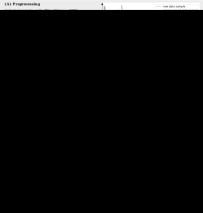
\includegraphics[width=1\textwidth]{img/remodnav_algorithm.pdf}
  \caption{\remodnav workflow. Optional steps and configurable parameters are bold.}
  \label{fig:alg}
\end{figure*}

All available parameters (sorted by algorithm step) with their description and,
if applicable, default value, are listed in table \ref{tab:parameters} and
displayed in figure \ref{fig:alg}. While input required by the user is minimal
(raw data, sampling rate, viewing distance and screen size), the amount of
configurable parameters may seem large. However, this is implemented
purposefully.  The available literature on eye event detection algorithms
suggests that there is no true ``one-fits-all" solution for event detection.
There are some successful approaches using deep neural networks
\citep{Startsev2018}, but those need appropriately large amounts of suitable
training data, that may not be easily available. As evident from many
evaluations and applications of algorithms (e.g. \cite{Andersson2017},
\cite{Larsson2013}, \cite{Zemblys2018}, \cite{5523936}), different underlying
stimulation, data characteristics, or use cases make certain algorithms more
suitable than others, hard-coded thresholds and parameters either applicable or
detrimental, or potentially require changes to the default values or
parameters. For our own analyses, the default parameter values were well
applicable. But we cannot anticipate how the data from other groups or
paradigms looks like.  \remodnav therefore contains a broad range of
transparent, interpretable and adjustable parameters with default values
justified from physiological findings or biological limitations, and no
hard-coded values. This gives users an option to adjust the algorithm to their
data's characteristics, but offers a sensible starting point with defaults that
proved to work well with the different datasets we evaluated the algorithm on.
Only velocity thresholds for saccade detection are estimated iteratively from
the data. Apart from the advantage of taking noise levels into account, this
also follows the reasoning of \cite{Nystrom2010AnData} that uninformed
adjustments of this parameter can have vast consequences on saccade detection,
and, subsequently, the labeling of all other eye events.

\begin{table*}[t]
  \caption{Algorithm parameters and their default values
  \todo[inline]{recall citation for choosing value of max\_initial\_saccade\_freq, pursuit\_velthresh}}
  \label{tab:parameters}
  \small
  \begin{tabular}{lp{85mm}l}
    \textbf{Name} & \textbf{Description} & \textbf{Value} \\
    & & \\
    \multicolumn{3}{l}{\textit{Preprocessing (in order of application during processing)}} \\
    \texttt{px2deg} &
    size of a single (square) pixel in degrees of visual angle &
    no default [\unit{deg/s}]\\
    \texttt{sampling\_rate} &
    temporal data sampling rate/frequency &
    no default [\unit{Hz}]\\
    \texttt{min\_blink\_duration} &
    missing data windows shorter than this duration will not be considered for \texttt{dilate\_nan}&
    \unit[0.02]{s}\\
    \texttt{dilate\_nan} &
    duration for which to replace data by missing data markers on either side of a
    signal-loss window &
    \unit[0.01]{s}\\
    \texttt{median\_filter\_length} &
    smoothing median-filter size (for initial data chunking only) &
    \unit[0.05]{s}\\
    \texttt{savgol\_length} &
    size of Savitzky-Golay filter for noise reduction&
    \unit[0.019]{s}\\
    \texttt{savgol\_polyord} &
    polynomial order of Savitzky-Golay filter for noise reduction&
    2\\
    \texttt{max\_vel} &
    maximum velocity threshold, will issue warning if exceeded to inform about
    potentially inappropriate filter settings&
    \unit[1000]{deg/s}\\

    \\\multicolumn{3}{l}{\textit{Event detection}} \\
    \texttt{min\_saccade\_duration} &
    minimum duration of a saccade event candidate &
    \unit[0.01]{s}\\
    \texttt{max\_pso\_duration} &
    minimum duration of a post-saccadic oscillation (glissade) candidate &
    \unit[0.04]{s}\\
    \texttt{min\_fixation\_duration} &
    minimum duration of a fixation event candidate &
    \unit[0.04]{s}\\
    \texttt{min\_pursuit\_duration} &
    minimum duration of a pursuit event candidate &
    \unit[0.04]{s}\\
    \texttt{min\_intersaccade\_duration} &
    no saccade detection is performed in windows shorter than twice this value, plus minimum saccade and PSO duration&
    \unit[0.04]{s}\\
    \texttt{noise\_factor} &
    adaptive saccade onset threshold velocity is the median absolute deviation of velocities in the window of interest, times this factor (peak velocity threshold is twice the onset velocity); increase for noisy data to reduce false positives \citep[equivalent: 3.0]{Nystrom2010AnData}&
    5\\
    \texttt{velthresh\_startvelocity} &
    start value for adaptive velocity threshold algorithm \citep{Nystrom2010AnData}, should
    be larger than any conceivable minimum saccade velocity &
    \unit[300]{deg/s}\\
    \texttt{max\_initial\_saccade\_freq} &
    maximum saccade frequency for initial detection of major saccades, initial data
    chunking is stopped if this frequency is reached (should be smaller than an expected
    (natural) saccade frequency in a particular context)&
    \unit[2]{Hz}\\
    \texttt{saccade\_context\_window\_length} &
    size of a window centered on any velocity peak for adaptive determination of
    saccade velocity thresholds (for initial data chunking only) &
    \unit[1]{s}\\
    \texttt{lowpass\_cutoff\_freq} &
    cut-off frequency of a Butterworth low-pass filter applied to determine drift
    velocities in a pursuit event candidate &
    \unit[4]{Hz}\\
    \texttt{pursuit\_velthresh} &
    fixed drift velocity threshold to distinguish periods of pursuit from periods of fixation &
    \unit[2]{deg/s}\\
  \end{tabular}
\end{table*}


% \todo[inline]{did we enforce a minimum saccade duration?} Yes, looks like it (Adina)

%\subsection*{Going beyond basic dynamic stimuli; the studyforrest dataset}
%\todo[inline]{\textit{fix/update text below}}

%\todo[inline]{this sections describes the method that produces the
%data artifacts. what kind of filtering? What kind of saccade detection algorithm? It should contain an \textbf{ultra-brief} summary of the eyetracking details from \cite{HAK+16}, but otherwise just refer to this article for details.}

%In the original study, Hanke et. al \cite{Hanke.2016} split 30 participants into groups of 15 and placed one half in a fMRI scanner set-up and the other in a lab setting while recording eye movements during the two hour movie stimulus. For further technical details please refer to the original article. As part of an unpublished Bachelor project, we compared different filter and saccade detection algorithm combinations. To quantify the precision of the combination, the correlation between peak velocity and amplitude of all saccades, known as the main sequence, and the inherent $r^2$ values were computed. The higher the data fit to the assumed main sequence $MS$ curve $MS=mx^n$ the more precise the filter-algorithm option. The combination of Savitzky-Golay filter and an adaptive detection algorithm by Nyström and Holmqvist proved to be most precise and was used for further analysis. The respective algorithm employs a daten-driven threshold which automatically adjusts to local noise levels. It consists of five steps including filtering with Savitzgy-Golay, peak saccade detection, saccade on- and offset determination, as well as glissade and fixation identification. Parameters used for computation were kept exactly as suggested by the authors. According to the algorithm, after detecting saccades and follow-up glissades, the left over movements between saccades were considered fixations. Due to higher noise in dynamic stimuli and the longer recording period this assumption did not hold in the studyforrest dataset. Therefore, an additional velocity limit of 6.58 $\frac{\circ}{s}$ and amplitude of 2 $^\circ$ during a fixation was integrated as these values are commonly viewed as fixation thresholds.\cite{Holmqvist.2011,Henderson.1997}

%Methods should include a brief discussion of allowances made (if any) for controlling bias or unwanted sources of variability, and the limitations of the datasets.



%\todo[inline]{\textit{brief description of the nature and amount of data released, and in which format it is released in}}
%The data is divided into lab and scanner data and released as separate text files for each movie segment per participant. This results in a set of 240 .txt files. The first step of the detection process includes disregarding biologically implausible values and blinks followed up by  Savitzky-Golay filtering. The output files display the velocity, acceleration, point in time and pixel coordinates for each sample and are released separately to enable additional calculations. These files are then further processed to detect saccades, glissades and fixations. The final output includes the typical eye tracking information on each movement event: time and coordinates for on- and offset, amplitude, peak velocity and average velocity. (peak velocity was not calculated for fixations)

\subsection*{Operation}\label{op}

\remodnav\ is free and open-source software, written in the Python language and
released under the terms of the MIT license. In addition to the Python standard
library it requires the Python packages
%
NumPy \citep{oliphant2006guide},
Matplotlib \citep{hunter2007matplotlib},
statsmodels \citep{seabold2010statsmodels},
and SciPy \citep{JOP+2001} as software dependencies.
Furthermore, DataLad \citep{HH+2013},
and Pandas \citep{mckinney2010data}
%
have to be available for assessing correct operation via the \remodnav test
battery. \remodnav itself, and all software dependencies are available on all
major operating systems.  There are no particular hardware requirements for
running the software other than sufficient memory to load and process the data.


\section*{Validation analyses}\label{ana}

% \todo[inline]{three major types of comparison: with andersson human labeling,
% stats of forrest lab recording with andersson video data stats, forrest lab
% vs forrest mri stats. the goal is to show that we are similar to humans, as
% good (or better) as other algorithms (by comparison with scores in
% andersson2017), and proceduce "similar" results on a different movie dataset,
% and similar results across two different qualities of recordings with the
% same stimulus (lab vs MRI). No more, no less IMHO. This all translates to
% three use cases: trial-by-trial data (from anderson), good movie data without
% trial structure (forrest lab), bad movie data (forrest mri)}

% THIS SECTION  WILL BASICALLY SHOW THE INPUTS AND THE OUTPUTS(RESULTS
% BASICALLY)

% \todo[inline]{\textit{Testing and comparison --- explaining rationale of the
% compared algorithms ie they were winners in the anderson paper}}

We applied our algorithm to two datasets, each to fulfill different objectives.
First, in order to validate REMoDNaV, we used the manually annotated dataset
from the Humanities Lab, Lund University, used by
\cite{Andersson2017}\footnote{github.com/richardandersson/EyeMovementDetector\linebreak[0]Evaluation},
to see how our algorithm compared against the NH algorithm it is based on and
manual human annotation of eye gaze events. This was done to verify that
changes introduced in \remodnav do not decrease performance below that of the
NH algorithm, and to evaluate whether REMoDNaV indeed improves eye movement
detection during dynamic stimulation as intended, compared to ten contemporary
event detection algorithms. Secondly, we used our algorithm on the studyforrest
dataset \citep{Hanke2016} to see the results of dynamic stimuli under two
different noise conditions: A high-quality dataset from a laboratory setting,
and low-quality data from a simultaneous fMRI and eye gaze acquisition.  This
analysis aims to provide an estimate of the robustness of the algorithm results
and follows a simple reasoning: As the stimulus (the Hollywood movie: Forrest
Gump) is the same in both noise conditions, it should evoke similar gaze
characteristics regardless of the quality of its measurement. Should \remodnav
extract similar eye event properties, then this is a good indicator of robust
performance even under high noise conditions.

\subsection*{Evaluation of the algorithm: comparing outputs against human
coders and a current algorithm}\label{ana_1}

The dataset provided by \cite{Andersson2017} consists of monocular eye gaze
data produced from viewing stimuli from three distinct categories -- images,
moving dots and videos. In addition to the eye tracking metadata (eye tracker
sampling rate (500hz), size of the screen, raw eye gaze data, distance from
screen) and eye gaze data (coordinates), each frame was also labeled by two
human observers to assign the event they thought it was. A total of six
different labels were used, namely, fixation, saccade, post-saccadic
oscillation, smooth pursuit, blink and undefined (a sample that did not fit any
other category). A minor labeling mistake reported in \cite{Zemblys2018} was
fixed prior to the computations.

To compare the REMoDNaV results to the human coders and the performance of the
NH algorithm, we applied \remodnav to the Humanities lab dataset and followed
the approach by \citet{Andersson2017}: For one, for each stimulus category, we
computed the proportion of misclassification per event type compared to each of
the human coders, and compared human coders against each other. A time point
classified by \remodnav counted as ``misclassified" if the associated event did
not correspond to the label the human coder assigned. We limited this analysis
to all time points that have been labeled as fixation, saccade, PSO, or pursuit
by any method, hence ignoring the rarely used NaN/blinks or ``undefined"
category. In order to provide a comparison to NH and the other algorithms in
\cite{Andersson2017}, this misclassification analysis was repeated excluding
samples labeled as pursuit (as none of the algorithms classed this category).
The results of this analysis are displayed in table \ref{tab:mclf}. For the
comparison performed by \citet{Andersson2017}, the NH algorithm disagreed with
human coders in 32\% of samples for images, in 93\% of samples for moving dots,
and in 70\% of samples for videos. In a direct comparison, i.e. if smooth
pursuit movements are not taken into account, our algorithm had a lower
misclassification rate. The highest disagreement across all stimuli categories
and coders is 11.7\%. Compared to all ten algorithms used in
\citet{Andersson2017}, \remodnav displays the lowest misclassification rates in
all categories

When taking smooth pursuit movements into account, the misclassification ratio
increases, as would be expected with the introduction of a fourth eye movement
category. Importantly, despite an increase, the misclassification rate remains
comparably low, thus still exceeding the performance of all contemporary
algorithms in \citet{Andersson2017} in the dynamic categories dots and videos.
For a comparison between algorithm and human coders classification, figure
\ref{fig:conf} displays the resulting confusion matrices with Jaccard indices
(JI) quantifying the similarity between classification decisions. The JI is
bound in range [0, 1] with higher values indication higher similarity. A value
of 0.93 in the upper left cell of the very first matrix in figure
\ref{fig:conf} for example indicates that 93\% of frames that are labeled as a
fixation by human coders RA and MN are the same. This index allows to quantify
the similarity of classifications independent from values in other cells. While
the highest similarity in labeling (evident from high values along the
diagonal) exists between human coders, the algorithm still performs well. For
the new event type smooth pursuit, detection is very consistent to human labels
especially in the moving dot category (JI of .73 and .7, respectively), and
still good in the video category (JI of .43 and .47, respectively)

\begin{table}[h!]
  % table caption is above the table
  \caption{Confusion matrices for different stimulus categories}
  \label{tab:mclf}       % Give a unique label
  % For LaTeX tables use
  \begin{tabular}{llllllll}
    \textbf{Images}&&&&&&&\\
    \hline\noalign{\smallskip}
    Comp & MC & w/oP & Coder & Fix & Sac & PSO & SP \\
    \noalign{\smallskip}\hline\noalign{\smallskip}
    MN-RA & \imgMNRAMCLF & \imgMNRAMclfWOP & MN & \imgMNRAFIXref & \imgMNRASACref & \imgMNRAPSOref & \imgMNRASPref  \\
    --- & --- & --- & RA & \imgMNRAFIXcod & \imgMNRASACcod & \imgMNRAPSOcod & \imgMNRASPcod \\
    MN-AL & \imgMNALGOMCLF & \imgMNALGOMclfWOP & MN & \imgMNALGOFIXref & \imgMNALGOSACref & \imgMNALGOPSOref & \imgMNALGOSPref \\
    --- & --- & --- & AL & \imgMNALGOFIXcod & \imgMNALGOSACcod & \imgMNALGOPSOcod & \imgMNALGOSPcod \\
    RA-AL & \imgRAALGOMCLF & \imgRAALGOMclfWOP & RA & \imgRAALGOFIXref & \imgRAALGOSACref & \imgRAALGOPSOref & \imgRAALGOSPref \\
    ---& ---& ---& AL & \imgRAALGOFIXcod & \imgRAALGOSACcod & \imgRAALGOPSOcod & \imgRAALGOSPcod \\
    \noalign{\smallskip}
    \textbf{Dots}&&&&&&&\\
    \hline\noalign{\smallskip}
    Comp & MC & w/oP & Coder & Fix & Sac & PSO & SP \\
    \noalign{\smallskip}\hline\noalign{\smallskip}
    MN-RA & \dotsMNRAMCLF & \dotsMNRAMclfWOP & MN & \dotsMNRAFIXref & \dotsMNRASACref & \dotsMNRAPSOref & \dotsMNRASPref  \\
    --- & --- & --- & RA & \dotsMNRAFIXcod & \dotsMNRASACcod & \dotsMNRAPSOcod & \dotsMNRASPcod \\
    MN-AL & \dotsMNALGOMCLF & \dotsMNALGOMclfWOP & MN & \dotsMNALGOFIXref & \dotsMNALGOSACref & \dotsMNALGOPSOref & \dotsMNALGOSPref \\
    --- & --- & --- & AL & \dotsMNALGOFIXcod & \dotsMNALGOSACcod & \dotsMNALGOPSOcod & \dotsMNALGOSPcod\\
    RA-AL & \dotsRAALGOMCLF & \dotsRAALGOMclfWOP & RA & \dotsRAALGOFIXref & \dotsRAALGOSACref & \dotsRAALGOPSOref & \dotsRAALGOSPref \\
    ---& ---& ---& AL & \dotsRAALGOFIXcod & \dotsRAALGOSACcod & \dotsRAALGOPSOcod & \dotsRAALGOSPcod \\
    \noalign{\smallskip}
    \textbf{Videos}&&&&&&&\\
    \hline\noalign{\smallskip}
    Comp & MC & w/oP & Coder & Fix & Sac & PSO & SP \\
    \noalign{\smallskip}\hline\noalign{\smallskip}
    MN-RA & \videoMNRAMCLF & \videoMNRAMclfWOP & MN & \videoMNRAFIXref & \videoMNRASACref & \videoMNRAPSOref & \videoMNRASPref \\
    --- & --- & --- & RA & \videoMNRAFIXcod & \videoMNRASACcod & \videoMNRAPSOcod & \videoMNRASPcod \\
    MN-AL & \videoMNALGOMCLF & \videoMNALGOMclfWOP & MN & \videoMNALGOFIXref & \videoMNALGOSACref & \videoMNALGOPSOref & \videoMNALGOSPref \\
    --- & --- & --- & AL & \videoMNALGOFIXcod & \videoMNALGOSACcod & \videoMNALGOPSOcod & \videoMNALGOSPcod\\
    RA-AL & \videoRAALGOMCLF & \videoRAALGOMclfWOP & RA & \videoRAALGOFIXref & \videoRAALGOSACref & \videoRAALGOPSOref & \videoRAALGOSPref \\
    ---& ---& ---& AL & \videoRAALGOFIXcod & \videoRAALGOSACcod & \videoRAALGOPSOcod & \videoRAALGOSPcod \\
    \noalign{\smallskip}\hline
  \end{tabular}

  \textit{Note}: Proportion of samples in in the image category classified in
  disagreement within the human coders (MN-RA) or between \remodnav algorithm
  (AL) and one human coder. The MC (misclassification) column indicates the
  proportion of samples where the human coders disagreed with each other, or
  where the algorithm disagreed with a human coder. The w/oP (without pursuit)
  column is the same measure, but excludes all pursuit samples. The remaining
  columns display the percentage of labels used in misclassified samples.
  Within each row, percentages per Coder should add up tp 100\%, in rare cases
  rounding leads to 99 or 101\%, though.

\end{table}

% Simple quick example of what I envision a confusion matrix graphic could look
% like.

\begin{figure*}
  % Use the relevant command to insert your figure file.
  % For example, with the graphicx package use
  % TODO make final figure and switch
  %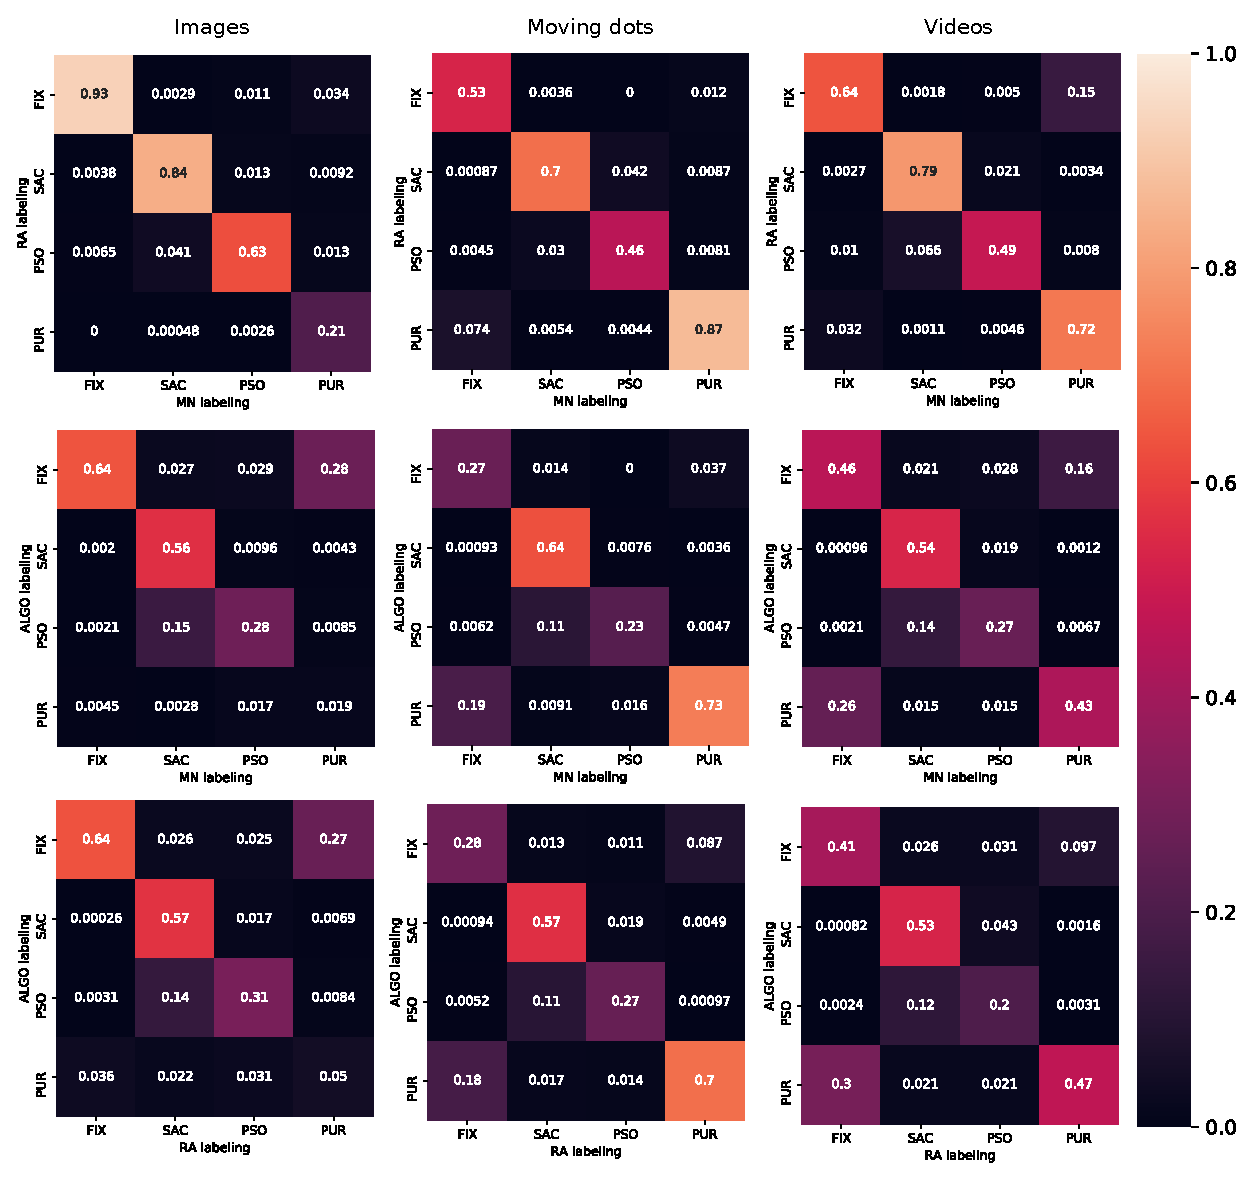
\includegraphics[width=1\textwidth]{img/conf_drawing.eps}
  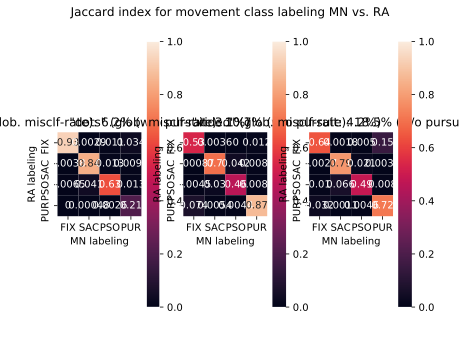
\includegraphics[width=1\textwidth]{img/confusion_MN_RA.pdf} \\
  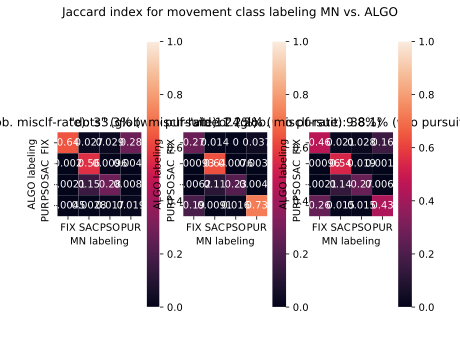
\includegraphics[width=1\textwidth]{img/confusion_MN_ALGO.pdf} \\
  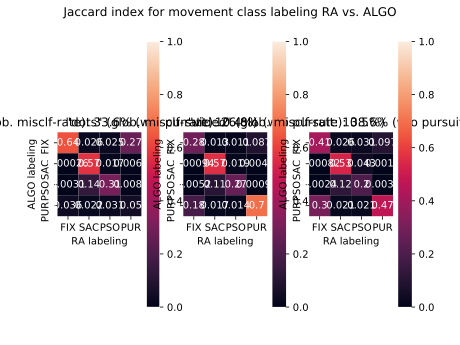
\includegraphics[width=1\textwidth]{img/confusion_RA_ALGO.pdf}
  % figure caption is below the figure
  \caption{Confusion matrices indicating similarity for classification decisions between human coders (top panel),
  human coder MN and \remodnav (middle panel), and human coder RA and \remodnav (bottom panel) for each of the
  three stimulus categories. Numbers denote Jaccard indices (higher is more similar).}
  \label{fig:conf}
  % Give a unique label
\end{figure*}

%\begin{figure*}[!ht]
%\centering
%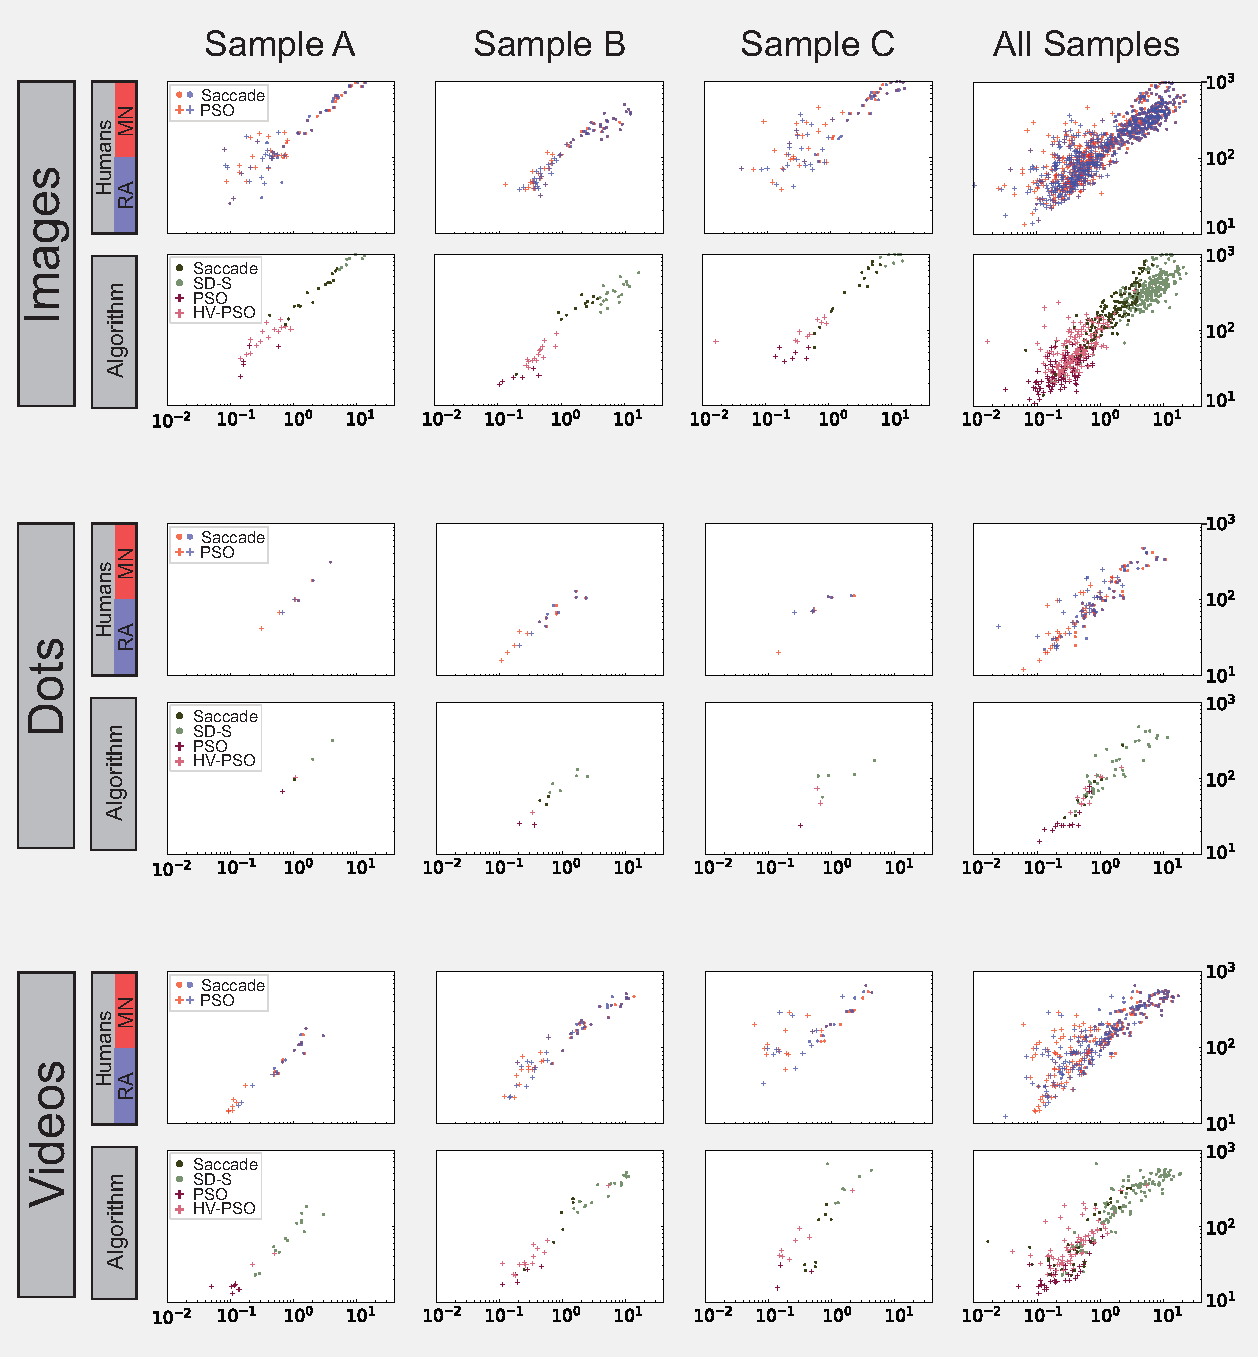
\includegraphics[width=1\textwidth]{Mainseqs_legends.pdf}
%\caption{\label{fig:Mainseqs}Overview of use cases to validate to anderson dataset. Three sets of stimuli, namely, images, dots, and videos which are processed by human observers and the algorithm. Sample A shows results that show a good match between the human and algorithmic results,sample B showing acceptable results, while sample C shows a poor match. In the case of the human observers the results of each observer --- represented by either blue or red --- are superimposed onto one another. Event detection done by the algorithm additionally split saccadic events into Segment defining saccades (SD-S) and PSOs to regular and High velocity PSOs (HV-PSO)  }

%\end{figure*}

Additionally, for each stimulus category (images, dots, videos), we determined
the mean and standard deviation of the event durations per event category (fixations,
saccades, PSOs, pursuits) and the number of detected events per event category.
Based on these results, following equation 2 in \citet{Andersson2017}, we computed
the root mean squared deviations (RMSD) for the full set of algorithms, human coders,
and REMoDNav. The RMSD is proposed by \cite{Andersson2017} as a single similarity
measure of distribution parameters to rank algorithms according to their similarity
to human coders in three dimensions. As \citet{Andersson2017} point out, this measure
ensures that we do not only evaluate performance on a sample-by-sample classification
similarity, but also evaluate whether an algorithm detects similar event counts and
duration distributions.
The RMSD measure has a lower bound of 0 and higher values denote
higher deviations, but for a thorough explanation of the measure and the procedures
necessary for its computation, please refer to the original publication by
\cite{Andersson2017}. By computing the RMSD of \remodnav within the original set
of data from \citet{Andersson2017}, we are able to compare the similarity of the
three distribution parameters produced by \remodnav to human labeling and those of
the other algorithms, and thus rank \remodnav within the set of algorithms used in
\citet{Andersson2017}.
For a more straightforward interpretation of the RMSD measure, we converted
RMSDs per event and stimulus category into ranks (where 0 is the best).
The results of the RMSD computations are summarized in tables \ref{tab:rmsd_fix},
\ref{tab:rmsd_sac}, \ref{tab:rmsd_pso} and \ref{tab:rmsd_pur}.
The "best" algorithm with regard to saccade and PSO detection in \cite{Andersson2017}
was the ``LNS" algorithm by \cite{Larsson2013}. \remodnav performs comparable to
``LNS" for saccades: Across stimulus categories, ``LNS" achieves a mean rank of $2.0$,
while \remodnav achieves a mean rank of $3.3$. For PSOs, across
stimulus categories, ``LNS" has a mean rank of $2.3$, while \remodnav achieves a
mean rank of $2.0$.
In the original set, different algorithms performed best for fixation detection
given the category. NH performed best for images  and videos, but worst for dots.
In our evaluation, \remodnav outperforms all other
algorithms in the dots category, and achieves rank 5 and 6 for videos and images,
respectively. That is, for fixation detection in videos and images, \remodnav
performs in the middle range. Across all stimulus and event categories,
\remodnav achieves a median ranking of $3.0$ (both with and without inclusion of
its ranks for smooth pursuit detection). Thus, \remodnav detects the number
of events and their duration distribution consistently similar to human coders,
especially so for saccades and PSOs, and fixations in the dots category.


\begin{table*}[h!]
  % table caption is above the table
  \caption{RMSD ranks of fixation parameters for various stimulation types}
  \label{tab:rmsd_fix}       % Give a unique label
  % For LaTeX tables use
  \begin{tabular*}{\textwidth}{c @{\extracolsep{\fill}}lllllllllllll}
    \hline\noalign{\smallskip}
    & \multicolumn{4}{l}{Images} & \multicolumn{4}{l}{Dots} & \multicolumn{4}{l}{Videos}\\
    Algorithm & Mean & SD & \# & rank &  Mean & SD & \# & rank & Mean & SD & \# & rank \\
    \noalign{\smallskip}\hline\noalign{\smallskip}
    MN        & \FIXimgmnMN   & \FIXimgsdMN   & \FIXimgnoMN   & \rankFIXimgMN   &  \FIXdotsmnMN   & \FIXdotssdMN   & \FIXdotsnoMN   & \rankFIXdotsMN    & \FIXvideomnMN   & \FIXvideosdMN   & \FIXvideonoMN   & \rankFIXvideoMN    \\
    RA        & \FIXimgmnRA   & \FIXimgsdRA   & \FIXimgnoRA   & \rankFIXimgRA   &  \FIXdotsmnRA   & \FIXdotssdRA   & \FIXdotsnoRA   & \rankFIXdotsRA    & \FIXvideomnRA   & \FIXvideosdRA   & \FIXvideonoRA   & \rankFIXvideoRA    \\
    CDT       & \FIXimgmnCDT  & \FIXimgsdCDT  & \FIXimgnoCDT  & \rankFIXimgCDT  &  \FIXdotsmnCDT  & \FIXdotssdCDT  & \FIXdotsnoCDT  & \rankFIXdotsCDT   & \FIXvideomnCDT  & \FIXvideosdCDT  & \FIXvideonoCDT  & \rankFIXvideoCDT   \\
    EM        & -             & -             & -             & -               &  -              & -              & -              & -                 & -               & -               & -               & -                  \\
    IDT       & \FIXimgmnIDT  & \FIXimgsdIDT  & \FIXimgnoIDT  & \rankFIXimgIDT  &  \FIXdotsmnIDT  & \FIXdotssdIDT  & \FIXdotsnoIDT  & \rankFIXdotsIDT   & \FIXvideomnIDT  & \FIXvideosdIDT  & \FIXvideonoIDT  & \rankFIXvideoIDT   \\
    IKF       & \FIXimgmnIKF  & \FIXimgsdIKF  & \FIXimgnoIKF  & \rankFIXimgIKF  &  \FIXdotsmnIKF  & \FIXdotssdIKF  & \FIXdotsnoIKF  & \rankFIXdotsIKF   & \FIXvideomnIKF  & \FIXvideosdIKF  & \FIXvideonoIKF  & \rankFIXvideoIKF   \\
    IMST      & \FIXimgmnIMST & \FIXimgsdIMST & \FIXimgnoIMST & \rankFIXimgIMST &  \FIXdotsmnIMST & \FIXdotssdIMST & \FIXdotsnoIMST & \rankFIXdotsIMST  & \FIXvideomnIMST & \FIXvideosdIMST & \FIXvideonoIMST & \rankFIXvideoIMST  \\
    IHMM      & \FIXimgmnIHMM & \FIXimgsdIHMM & \FIXimgnoIHMM & \rankFIXimgIHMM &  \FIXdotsmnIHMM & \FIXdotssdIHMM & \FIXdotsnoIHMM & \rankFIXdotsIHMM  & \FIXvideomnIHMM & \FIXvideosdIHMM & \FIXvideonoIHMM & \rankFIXvideoIHMM  \\
    IVT       & \FIXimgmnIVT  & \FIXimgsdIVT  & \FIXimgnoIVT  & \rankFIXimgIVT  &  \FIXdotsmnIVT  & \FIXdotssdIVT  & \FIXdotsnoIVT  & \rankFIXdotsIVT   & \FIXvideomnIVT  & \FIXvideosdIVT  & \FIXvideonoIVT  & \rankFIXvideoIVT   \\
    NH        & \FIXimgmnNH   & \FIXimgsdNH   & \FIXimgnoNH   & \rankFIXimgNH   &  \FIXdotsmnNH   & \FIXdotssdNH   & \FIXdotsnoNH   & \rankFIXdotsNH    & \FIXvideomnNH   & \FIXvideosdNH   & \FIXvideonoNH   & \rankFIXvideoNH    \\
    BIT       & \FIXimgmnBIT  & \FIXimgsdBIT  & \FIXimgnoBIT  & \rankFIXimgBIT  &  \FIXdotsmnBIT  & \FIXdotssdBIT  & \FIXdotsnoBIT  & \rankFIXdotsBIT   & \FIXvideomnBIT  & \FIXvideosdBIT  & \FIXvideonoBIT  & \rankFIXvideoBIT   \\
    LNS       & -             & -             & -             &  -              &  -              & -              & -              &  -                & -               & -               & -               &  -                 \\
    \remodnav & \FIXimgmnRE   & \FIXimgsdRE   & \FIXimgnoRE   & \rankFIXimgRE   &  \FIXdotsmnRE   & \FIXdotssdRE   & \FIXdotsnoRE   & \rankFIXdotsRE    & \FIXvideomnRE   & \FIXvideosdRE   & \FIXvideonoRE   & \rankFIXvideoRE    \\
    \noalign{\smallskip}\hline
  \end{tabular*}

  \textit{Note}: Fixation distribution parameters for the algorithms
  reported in \citet{Andersson2017} and \remodnav (bottom row). RMSDs
  were converted into ranks (lower is better).

\end{table*}

\begin{table*}[h!]
  % table caption is above the table
  \caption{RMSD ranks of saccade parameters for various stimulation types}
  \label{tab:rmsd_sac}       % Give a unique label
  % For LaTeX tables use
  \begin{tabular*}{\textwidth}{c @{\extracolsep{\fill}}lllllllllllll}
    \hline\noalign{\smallskip}
    & \multicolumn{4}{l}{Images} & \multicolumn{4}{l}{Dots} & \multicolumn{4}{l}{Videos}\\
    Algorithm & Mean & SD & \# & rank &  Mean & SD & \# & rank & Mean & SD & \# & rank \\
    \noalign{\smallskip}\hline\noalign{\smallskip}
    MN        & \SACimgmnMN   & \SACimgsdMN   & \SACimgnoMN   & \rankSACimgMN   &  \SACdotsmnMN   & \SACdotssdMN   & \SACdotsnoMN   & \rankSACdotsMN    & \SACvideomnMN   & \SACvideosdMN   & \SACvideonoMN   & \rankSACvideoMN    \\
    RA        & \SACimgmnRA   & \SACimgsdRA   & \SACimgnoRA   & \rankSACimgRA   &  \SACdotsmnRA   & \SACdotssdRA   & \SACdotsnoRA   & \rankSACdotsRA    & \SACvideomnRA   & \SACvideosdRA   & \SACvideonoRA   & \rankSACvideoRA    \\
    CDT       & -             & -             & -             & -               &  -              & -              & -              & -                 & -               & -               & -               & -                  \\
    EM        & \SACimgmnEM   & \SACimgsdEM   & \SACimgnoEM   & \rankSACimgEM    &  \SACdotsmnEM   & \SACdotssdEM   & \SACdotsnoEM   & \rankSACdotsEM    & \SACvideomnEM   & \SACvideosdEM   & \SACvideonoEM   & \rankSACvideoEM    \\
    IDT       & \SACimgmnIDT  & \SACimgsdIDT  & \SACimgnoIDT  & \rankSACimgIDT  &  \SACdotsmnIDT  & \SACdotssdIDT  & \SACdotsnoIDT  & \rankSACdotsIDT   & \SACvideomnIDT  & \SACvideosdIDT  & \SACvideonoIDT  & \rankSACvideoIDT   \\
    IKF       & \SACimgmnIKF  & \SACimgsdIKF  & \SACimgnoIKF  & \rankSACimgIKF  &  \SACdotsmnIKF  & \SACdotssdIKF  & \SACdotsnoIKF  & \rankSACdotsIKF   & \SACvideomnIKF  & \SACvideosdIKF  & \SACvideonoIKF  & \rankSACvideoIKF   \\
    IMST      & \SACimgmnIMST & \SACimgsdIMST & \SACimgnoIMST & \rankSACimgIMST &  \SACdotsmnIMST & \SACdotssdIMST & \SACdotsnoIMST & \rankSACdotsIMST  & \SACvideomnIMST & \SACvideosdIMST & \SACvideonoIMST & \rankSACvideoIMST  \\
    IHMM      & \SACimgmnIHMM & \SACimgsdIHMM & \SACimgnoIHMM & \rankSACimgIHMM &  \SACdotsmnIHMM & \SACdotssdIHMM & \SACdotsnoIHMM & \rankSACdotsIHMM  & \SACvideomnIHMM & \SACvideosdIHMM & \SACvideonoIHMM & \rankSACvideoIHMM  \\
    IVT       & \SACimgmnIVT  & \SACimgsdIVT  & \SACimgnoIVT  & \rankSACimgIVT  &  \SACdotsmnIVT  & \SACdotssdIVT  & \SACdotsnoIVT  & \rankSACdotsIVT   & \SACvideomnIVT  & \SACvideosdIVT  & \SACvideonoIVT  & \rankSACvideoIVT   \\
    NH        & \SACimgmnNH   & \SACimgsdNH   & \SACimgnoNH   & \rankSACimgNH   &  \SACdotsmnNH   & \SACdotssdNH   & \SACdotsnoNH   & \rankSACdotsNH    & \SACvideomnNH   & \SACvideosdNH   & \SACvideonoNH   & \rankSACvideoNH    \\
    BIT       & -             & -             & -             & -               &  -              & -              & -              & -                 & -               & -               & -               & -                  \\
    LNS       & \SACimgmnLNS  & \SACimgsdLNS  & \SACimgnoLNS  & \rankSACimgLNS  &  \SACdotsmnLNS  & \SACdotssdLNS  & \SACdotsnoLNS  & \rankSACdotsLNS   & \SACvideomnLNS  & \SACvideosdLNS  & \SACvideonoLNS  & \rankSACvideoLNS   \\
    \remodnav & \SACimgmnRE   & \SACimgsdRE   & \SACimgnoRE   & \rankSACimgRE   &  \SACdotsmnRE   & \SACdotssdRE   & \SACdotsnoRE   & \rankSACdotsRE    & \SACvideomnRE   & \SACvideosdRE   & \SACvideonoRE   & \rankSACvideoRE    \\
    \noalign{\smallskip}\hline
  \end{tabular*}

  \textit{Note}: Saccade distribution parameters for the algorithms
  reported in \citet{Andersson2017} and \remodnav (bottom row). RMSDs
  were converted into ranks (lower is better).

\end{table*}

\begin{table*}[h!]
  % table caption is above the table
  \caption{RMSD ranks of PSO parameters for various stimulation types}
  \label{tab:rmsd_pso}       % Give a unique label
  % For LaTeX tables use
  \begin{tabular*}{\textwidth}{c @{\extracolsep{\fill}}lllllllllllll}
    \hline\noalign{\smallskip}
    & \multicolumn{4}{l}{Images} & \multicolumn{4}{l}{Dots} & \multicolumn{4}{l}{Videos}\\
    Algorithm & Mean & SD & \# & rank &  Mean & SD & \# & rank & Mean & SD & \# & rank \\
    \noalign{\smallskip}\hline\noalign{\smallskip}
    MN        & \PSOimgmnMN   & \PSOimgsdMN   & \PSOimgnoMN   & \rankPSOimgMN   &  \PSOdotsmnMN   & \PSOdotssdMN   & \PSOdotsnoMN   & \rankPSOdotsMN    & \PSOvideomnMN   & \PSOvideosdMN   & \PSOvideonoMN   & \rankPSOvideoMN    \\
    RA        & \PSOimgmnRA   & \PSOimgsdRA   & \PSOimgnoRA   & \rankPSOimgRA   &  \PSOdotsmnRA   & \PSOdotssdRA   & \PSOdotsnoRA   & \rankPSOdotsRA    & \PSOvideomnRA   & \PSOvideosdRA   & \PSOvideonoRA   & \rankPSOvideoRA    \\
    NH        & \PSOimgmnNH   & \PSOimgsdNH   & \PSOimgnoNH   & \rankPSOimgNH   &  \PSOdotsmnNH   & \PSOdotssdNH   & \PSOdotsnoNH   & \rankPSOdotsNH    & \PSOvideomnNH   & \PSOvideosdNH   & \PSOvideonoNH   & \rankPSOvideoNH    \\
    LNS       & \PSOimgmnLNS  & \PSOimgsdLNS  & \PSOimgnoLNS  & \rankPSOimgLNS  &  \PSOdotsmnLNS  & \PSOdotssdLNS  & \PSOdotsnoLNS  & \rankPSOdotsLNS   & \PSOvideomnLNS  & \PSOvideosdLNS  & \PSOvideonoLNS  & \rankPSOvideoLNS   \\
    \remodnav & \PSOimgmnRE   & \PSOimgsdRE   & \PSOimgnoRE   & \rankPSOimgRE   &  \PSOdotsmnRE   & \PSOdotssdRE   & \PSOdotsnoRE   & \rankPSOdotsRE    & \PSOvideomnRE   & \PSOvideosdRE   & \PSOvideonoRE   & \rankPSOvideoRE    \\
    \noalign{\smallskip}\hline
  \end{tabular*}

  \textit{Note}: PSO distribution parameters for the algorithms
  reported in \citet{Andersson2017} and \remodnav (bottom row). RMSDs
  were converted into ranks (lower is better).

\end{table*}

\begin{table*}[h!]
  % table caption is above the table
  \caption{RMSD ranks of pursuit parameters for various stimulation types}
  \label{tab:rmsd_pur}       % Give a unique label
  % For LaTeX tables use
  \begin{tabular*}{\textwidth}{c @{\extracolsep{\fill}}lllllllllllll}
    \hline\noalign{\smallskip}
    & \multicolumn{4}{l}{Images} & \multicolumn{4}{l}{Dots} & \multicolumn{4}{l}{Videos}\\
    Algorithm & Mean & SD & \# & rank &  Mean & SD & \# & rank & Mean & SD & \# & rank \\
    \noalign{\smallskip}\hline\noalign{\smallskip}
    MN        & \PURimgmnMN   & \PURimgsdMN   & \PURimgnoMN   & \rankPURimgMN   &  \PURdotsmnMN   & \PURdotssdMN   & \PURdotsnoMN   & \rankPURdotsMN    & \PURvideomnMN   & \PURvideosdMN   & \PURvideonoMN   & \rankPURvideoMN    \\
    RA        & \PURimgmnRA   & \PURimgsdRA   & \PURimgnoRA   & \rankPURimgRA   &  \PURdotsmnRA   & \PURdotssdRA   & \PURdotsnoRA   & \rankPURdotsRA    & \PURvideomnRA   & \PURvideosdRA   & \PURvideonoRA   & \rankPURvideoRA    \\
    \remodnav & \PURimgmnRE   & \PURimgsdRE   & \PURimgnoRE   & \rankPURimgRE   &  \PURdotsmnRE   & \PURdotssdRE   & \PURdotsnoRE   & \rankPURdotsRE    & \PURvideomnRE   & \PURvideosdRE   & \PURvideonoRE   & \rankPURvideoRE    \\
    \noalign{\smallskip}\hline
  \end{tabular*}

  \textit{Note}: Smooth pursuit distribution parameters for the algorithms
  reported in \citet{Andersson2017} and \remodnav (bottom row). RMSDs
  were converted into ranks (lower is better).

\end{table*}


The combined results of the analyses on the dataset used by
\citet{Andersson2017} demonstrate that \remodnav yields the highest congruency
to manual human annotation in any stimulus category on a sample-by-sample basis
compared to ten contemporary algorithms when detecting fixations, saccades,
and post-saccadic oscillations. Its performance stays good, and exceeds all other
algorithms performance in the dots and video category, when including smooth
pursuit detection as well. In this regard, the results reveal that REMoDNaVs
performance equals or exceeds those of the original NH. Taking the number of events
and their duration distribution into account, REMoDNaVs performance stays good.
Importantly \remodnav performs similar to human coders in almost all event
categories and stimulus types. NH outperforms it only for fixation detection
in the image and video category, however, in these categories \remodnav still
classifies comparatively well. Thus, \remodnav does improve the NH algorithm
in aspects that were  suboptimal, but does not diminish performance in NHs strong points.

%\subsubsection*{Evaluation of events}

\subsection*{Prolonged recordings of natural viewing}\label{ana_2}

% discuss inlab vs scanner data

% \todo[inline]{\textit{Need to determine exactly which plots and tables will
% go here}}

% \todo[inline]{\textit{This section contains the analysis of the main
% sequences -- which I assume is the meat of the thesis. The goal is to have as
% much information as possible be contained in figures and/or tables (and their
% captions). We don't pay for those, but we do pay for the main text body.}}

Given that \remodnav yields biologically plausible results for dynamic
stimulation as indicated by the previous results, we determined whether it is
capable of analyzing data from dynamic stimulation without a trial structure.
For this, we applied it to the high quality eye tracking dataset obtained from
15 subjects watching the movie in a laboratory setting. This analysis further
serves as a base line to compare results obtained from a lower quality
recording to. Eye movements in this high-quality dataset were recorded with an
Eyelink 1000 with a standard desktop mount (software version 4.51; SR Research
Ltd., Mississauga, Ontario, Canada) and a sampling rate of 1000Hz. The movie
stimulus was presented on a $522$x$294$mm LCD monitor at a resolution of $1920$
x $1280$px at a viewing distance of 85cm \citep{Hanke2016}.  The top panel in
figure \ref{fig:remodnav} displays the performance of \remodnav for a high
quality data sample. An individual main sequence for a lab subject is
displayed in the bottom right panel in figure \ref{fig:overallComp}. In order
to compare event detection between high and low quality sample, we computed
the event distribution parameters per event type and movie run. Figure
\ref{yettodo} displays these parameters for the high quality dataset.
\todo[inline]{make histograms}

\begin{figure*}[h!]
  % TODO make final figure and switch
  %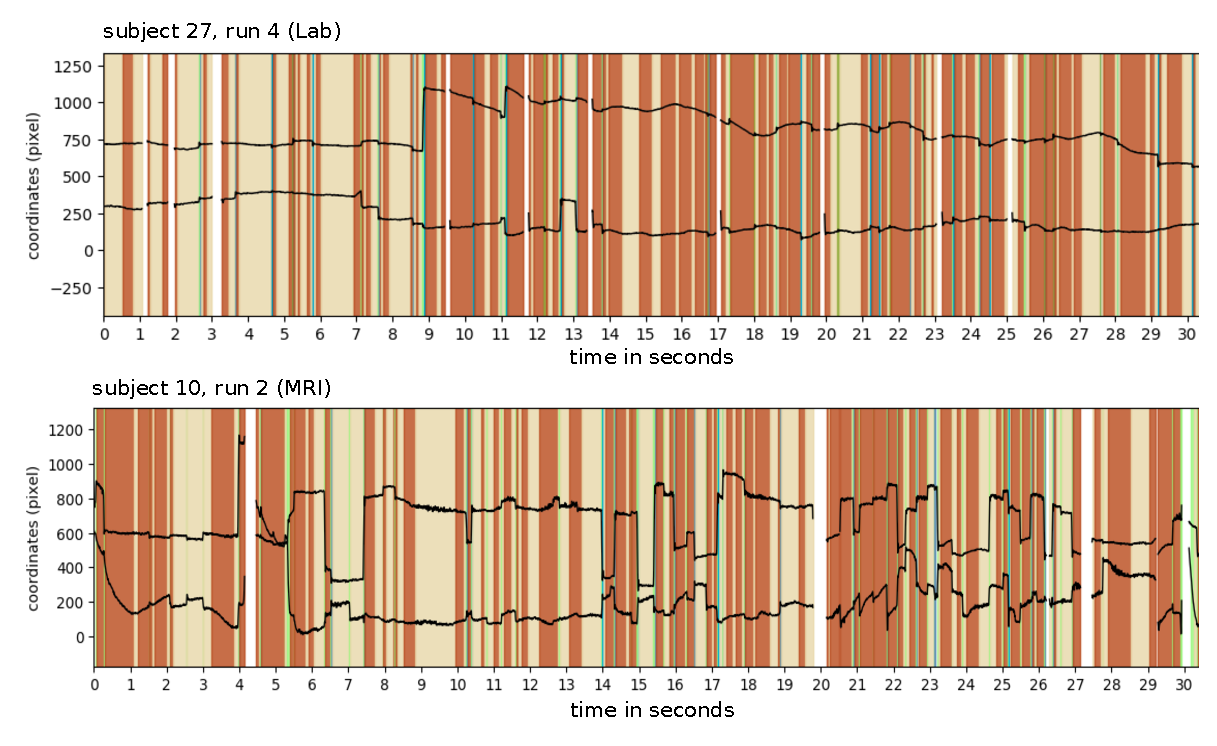
\includegraphics[width=1\textwidth]{img/remodnav.eps}
  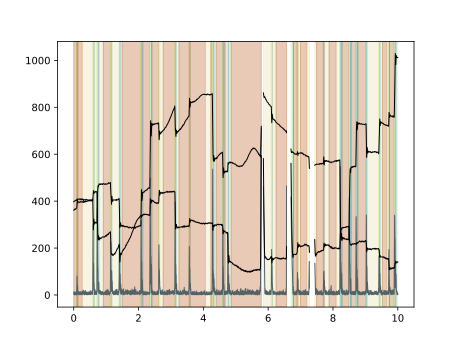
\includegraphics[trim=0 8.5mm 0 0,clip,width=1\textwidth]{img/remodnav_lab.pdf} \\
  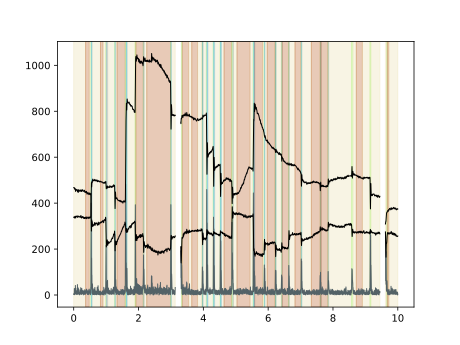
\includegraphics[trim=0 0 0 3.5mm,clip,width=1\textwidth]{img/remodnav_mri.pdf}\\
  \caption{Exemplary classification performance of \remodnav in a high quality lab sample (top panel) and low
  quality MRI sample (bottom panel), each for the same 10 seconds of movie stimulus.
  Black lines depict x and y coordinates of eye gaze, gray graph represents velocities. Colors indicate labeled
  eye events. Beige: Fixation,
  light green: Saccade, brown: Smooth pursuit, dark blue: High velocity PSOs, light blue: Low velocity PSOs.
  White: no signal}
  \label{fig:remodnav}
\end{figure*}

%\begin{figure*}[h!]
%  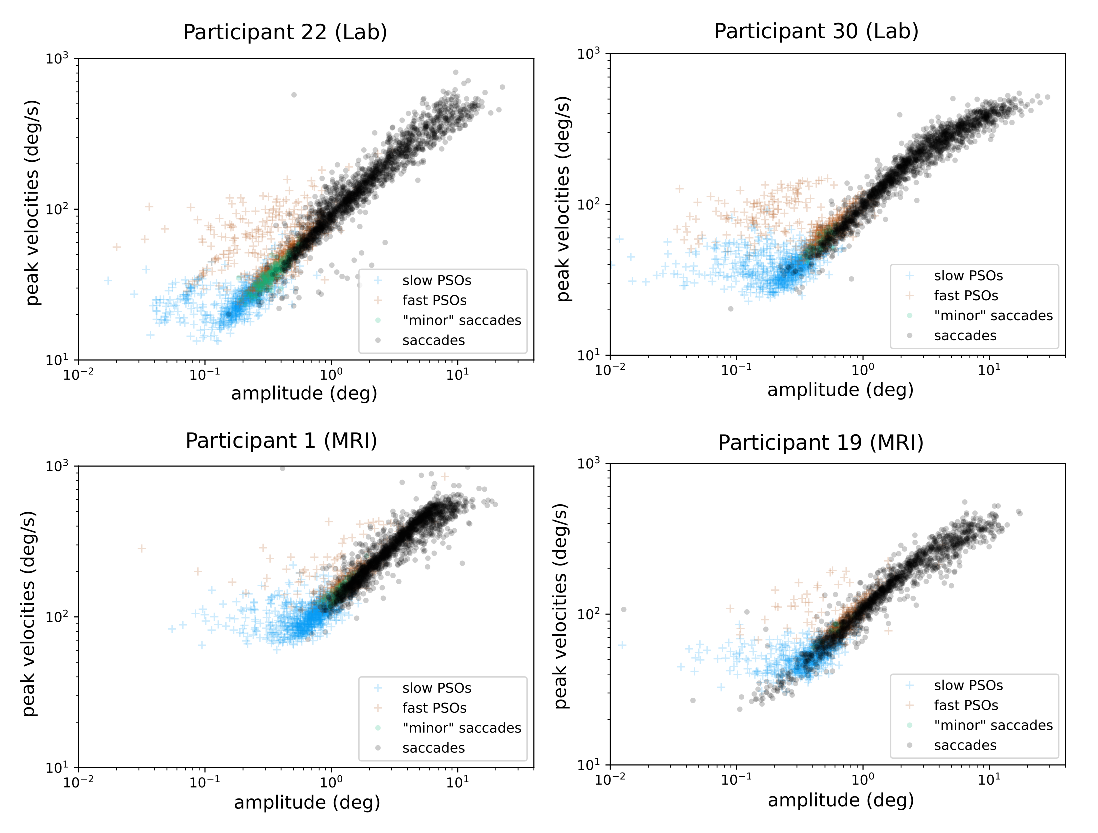
\includegraphics[width=1\textwidth]{img/main_sequences.eps}
%  \caption{Main sequences for four subjects, during one 15 minute sequence of
%  the movie. Top panel: Lab subjects, bottom panel: MRI subjects.}
%  \label{fig:mains}
%\end{figure*}

\subsection*{Low-quality data}\label{ana_3}

In order to determine the robustness of \remodnav to noise, in a last step, we
applied it to the low quality eye tracking dataset of the studyforrest
publication. This data was recorded with a different Eyelink 1000 (software
version 4.594) equipped with an MR-compatible telephoto lens and illumination
kit (SR Research Ltd., Mississauga, Ontario, Canada) at $1000$Hz during
simultaneous fMRI acquisition. The movie was presented at a viewing distance of
$63$cm on a 26cm ($1280$ x $1024$px) LCD screen in 720p resolution at full
width. The eye tracking camera was mounted outside the scanner bore and
recorded the participants left eye at a distance of about 100cm
\citep{Hanke2016}.  The lower data quality in this dataset is evident from a
generally higher amount of data loss and a larger spatial uncertainty (see
\citet{Hanke2016} for details on data quality). As the stimulus material was
the same between the high and low quality data sample, \remodnav demonstrates
robust performance if the characteristics of extracted events within the low
dataset correspond to those obtained from the previous high quality data
sample.

% N+H describe: "Data quality is related to accuracy, precision, percentage of
% data loss, perhaps in addition to a subjective rating from the person
% responsible for the recording"

Figure \ref{fig:remodnav} displays the performance of \remodnav for a low
quality data sample in the bottom row.  As evident in both panels, periods with
data loss do not interfere with the detection of eye movement events in their
vicinity beyond the border region of data loss that is masked during
preprocessing. The detection of saccades corresponds to the velocity peaks in
the time series. An individual main sequence for an MRI subject is displayed
in the top right panel in figure \ref{fig:overallComp}. Lastly, the left column in figure
\ref{fig:overallComp} shows all events produced from both datasets. Figure \ref{yettodo}
displays the distribution parameters per event type and movie run for the low
quality dataset. \todo[inline]{make histograms}
All together, figures \ref{fig:remodnav} and
\ref{fig:overallComp} illustrate a high similiarity between performance in high
and low quality datasets. In both cases, the main sequences follow the known
peak-velocity -- amplitude relationship of saccades. It is noteable that the
MRI sample displays fewer saccades of the shortest range. Given the higher
spatial uncertainty in this dataset, this is unsurprising: the eye tracker
likely was not able to capture these small eye movements under the low-light
conditions. Apart from this aspect, both main sequences are comparable. Given
that \remodnav classifies data from dynamic stimulation well, and that results
on low and high quality data yield similar biologically plausible results, the
performance seems to be robust even under high noise conditions.

\begin{figure*}[h!]
  \includegraphics[width=.5\textwidth]{img/mainseq_mri_300dpi.png}
  \includegraphics[width=.5\textwidth]{img/mainseq_sub_mri_300dpi.png} \\
  \includegraphics[width=.5\textwidth]{img/mainseq_lab_300dpi.png}
  \includegraphics[width=.5\textwidth]{img/mainseq_sub_lab_300dpi.png} \\

  \caption{Main sequence of eye movement events during one 15 minute sequence of
  the movie (segment 2) for MRI (top), and lab participants (bottom). Data
  across all participants is shown in the right, and data for a single
  exemplary participant on the left.}

  \label{fig:overallComp}
\end{figure*}


%
%\onecolumn
%
%%------------------figure------------------------------------------
%\begin{figure}
%\centering
%%\includegraphics[scale=0.35]{figures/MainSeq.png}
%        \caption[Main sequence plot]{Plot of the main sequence, relationship between peak velocity and amplitude of participant ID 24, movie segment 4 (randomly chosen as an example); $r^2$=0.92.}
%        \label{main}
%\end{figure}
%\begin{table}[h]
%\center
%\begin{tabular}{lcccc}
%\toprule
%\# & duration in $ms$  & amplitude in $^\circ$ & peak velocity in $\frac{^\circ} {s}$ & number of saccades \\
%\midrule
%1	& 	34.99$\pm$0.88 	& 	1.84$\pm$0.15   & 	102.78$\pm$5.43 	& 	884.9$\pm$205.0  	\\
%2 	& 	34.61$\pm$1.11 	&	2.22$\pm$0.16	&  	102.18$\pm$5.99		& 	897.3$\pm$72.1 		\\
%3	&   35.79$\pm$1.19	&   2.26$\pm$0.14 	&  	106.39$\pm$4.72		& 	901.93$\pm$192.9 	\\
%4 	& 	34.81$\pm$1.04 	&  	1.81$\pm$0.10 	& 	74.43$\pm$2.95		&	1148.7$\pm$191.2 	\\
%5 	& 	36.08$\pm$1.19 	&	2.48$\pm$0.17 	& 	97.17$\pm$3.83 		& 	899.0$\pm$240.3 	\\
%6	& 	35.09$\pm$0.78 	& 	1.82$\pm$0.09 	& 	111.79$\pm$3.86 	&	899.1$\pm$151.1 	\\
%7	& 	35.86$\pm$0.63	& 	1.87$\pm$0.10 	&  	89.88$\pm$3.45		& 	959.5$\pm$244.7		\\
%8	& 	34.22$\pm$0.64 	& 	2.55$\pm$0.37 	& 	128.48$\pm$11.09	& 	556.3$\pm$218.8		\\
%
%\bottomrule
%
%\end{tabular}
%\caption {Mean and standard deviations for different metrics grouped by the movie segment.}
%\label{rundetails1}
%\end{table}
%
%\begin{table}[h]
%
%\centering
%\scalebox{1}{
%\begin{tabular}{lcccc}
%\toprule
%\# & lost signal $\frac{s}{min}$ &$r^2$ & samples removed & slope\\
%
%\midrule
%1 & 4.7		& 	0.889 	&	7.9\%	&	0.510	\\
%2 & 3.8		&   0.856	&	7.0\%	&	0.578	\\
%3 & 5.4 	&   0.847	&	8.9\%	&	0.584	\\
%4 & 4.6 	& 	0.898	&	7.4\%	&	0.573	\\
%5 & 1.2 	& 	0.897	&	2.3\%	&	0.493	\\
%6 & 2.5 	& 	0.880	&	4.6\%	&	0.598	\\
%7 & 0.9 	& 	0.914	&	1.7\%	&	0.516	\\
%8 & 5.3 	&  	0.771	&	8.9\%	&	0.530	\\
%
%
%\bottomrule
%\end{tabular}}
%\caption{Movie segment analysis showing mean values for different metrics over every test subject in a run: Mean value of signal loss in seconds per minute , $r^2$ values for the correlation between peak velocity and amplitude, average percentage of samples removed, average slope of the main sequence. Due to blinks and noise, some samples were removed from the eye gaze data before calculations started. The average percentage of removed samples is illustrated. Across all participants 16\% was the maximum amount of samples neglected and in 93.3\% of the data less than 10\% were disregarded. Included in this removal was the actual pure signal loss during the recording session, meaning samples marked with a null value.}
%\label{rundetails2}
%\end{table}
%
%%------------------figure------------------------------------------
%\begin{figure}[h]
%\centering
%%\includegraphics[scale=0.2]{figures/duration.jpeg}
%        \caption{Histogram of saccade durations. Cut off at 100 $ms$ as for the following bars less than 0.01\% of all data are presented per bin, making it impossible to visualize. Normalized to 1. The largest amount of saccades is very close to minimum duration. The assumed shape of the distribution indicates a gradual decrease to the left, implying the possibility of a number of shorter, yet disregarded saccades. This loss of data can easily be fixed by choosing a less conservative duration threshold. There are many different subjective opinions on minimum saccadic duration, ranging from 10 ms \cite{Duchowski.2007} to 15 ms \cite{Smith.2013}. A more objective approach was provided by Carpenter in 1988 who found a mathematical relation between duration and amplitude of saccades \cite{Carpenter.1988}: $duration=2.2\cdot{}amplitude+21$. According to this equation there are no saccades of less than 21 $ms$. Therefore, a minimum duration of 21 $ms$ was chosen as threshold.}
%\label{dur}
%\end{figure}
%
%%------------------figure------------------------------------------
%\begin{figure}
%\centering
%%\includegraphics[scale=0.2]{figures/amp.jpeg}
%        \caption[Histogram of saccade amplitude]{Histogram of all saccade amplitudes. Cut off at 12 $^\circ$. Normalized to 1. }
%        \label{amp}
%\end{figure}
%
%%------------------figure------------------------------------------
%\begin{figure}
%\centering
%%\includegraphics[scale=0.2]{figures/pv.jpeg}
%        \caption[Histogram of peak velocity]{Histogram of all saccade peak velocities. Cut off at 400 $\frac{^\circ} {s}$. Normalized to 1. }
%        \label{pv}
%\end{figure}
%
%%------------------table------------------------------------------
%\begin{table}[h]
%
%\centering
%\scalebox{1}{
%\begin{tabular}{lcccccc}
%\toprule
%    \# & \multicolumn{3}{c}{glissades} & \multicolumn{2}{c}{fixations}\\
% & duration in $ms$ & amplitude in $^\circ$ & mean velocity in $\frac{^\circ} {s}$ & duration in $ms$ & number \\
%\midrule
%1	& 	39.68 	& 	0.13   	& 	6.60	& 	430.22	&	4965.1  \\
%2 	& 	39.70 	&	0.22	&  	10.93	& 	432.67	&	4865.5 	\\
%3	&   39.77	&   0.19 	&  	7.83	& 	429.49 	&	4975.5	\\
%4 	& 	39.73 	&  	0.09 	& 	5.41	&	394.11 	&	5802.3	\\
%5 	& 	39.73 	&	0.16 	& 	9.87 	& 	445.37 	&	4903.7	\\
%6	& 	39.72 	& 	0.16 	& 	11.65	&	435.96 	&	4823.7	\\
%7	& 	39.72	& 	0.09 	&  	4.92	& 	480.94	&	5403.7	\\
%8	& 	39.81 	& 	0.33 	& 	14.06	& 	469.67	&	3456.3	\\
%
%
%\bottomrule
%\end{tabular}}
%\caption[]{Movie segment analysis for glissades and fixations, showing mean values for different metrics over every test subject per segment, mean value of duration, amplitude, velocity, and number of fixations. Since glissade durations group around the cut off value of 40, it seems that most movements would have been longer than that. This indicates, that the threshold for glissade detection is too low, perceivably because the data used had a higher level of baseline noise than in the experiment by Nyström and Holmqvist.{\cite{Nystrom.2010}} Fixation durations range around a mean value of 420.42 $ms$. Typical values for fixations rarely exceed 400 $ms$. However, the significantly longer fixation durations align with the rest of the eye movements, as saccades were accordingly shorter than typical values suggest. Human gaze in general is preferably directed at the center of the stimulus {\cite{Buswell.1935,Parkhurst.2002}} and the pull towards the center was proven to be strongest in professionally cut Hollywood movie trailers when compared with natural scenes or static images. {\cite{Dorr.2010}} These findings supports the assumption, that participants mainly focused on the center of the screen, which is backed uo by the data. Fixations include small microsaccades, tremor and slow drifts, which allow the viewer to gradually explore the movie stimulus while staying within fixation parameter boundaries.}
%\label{fixgliss}
%\end{table}
%
%%------------------table-----------------------------------------
%\begin{table}[h]
%
%\centering
%\begin{tabular}{lcccccc}
%\toprule
%Movie segment & lab  & scanner & t-statistic & p-value \\
%\midrule
%\rowcolor{lightgray}
%1 	&	0.892 	&	0.740	& 	4.220	& 	0.0039	\\
%
%2	&   0.836 	&   0.841 	& 	0.242	& 	0.8156	\\
%
%3 	&   0.869 	& 	0.793	& 	2.797 	& 	0.0266	\\
%\rowcolor{lightgray}
%4 	&   0.892 	& 	0.590 	& 	7.115 	& 	0.0002	\\
%
%5 	&   0.912 	& 	0.883 	& 	3.789 	& 	0.0068	\\
%
%6 	&   0.917 	& 	0.771 	& 	2.700	& 	0.0306	\\
%
%7 	&   0.921 	& 	0.808 	& 	2.365 	& 	0.0500	\\
%
%8 	&   0.800 	& 	0.821 	& 	0.545	& 	0.6029	\\
%\bottomrule
%
%
%
%\end{tabular}
%\caption[]{Group comparison of lab and scanner data in regard of average $r^2$-value of the main sequence and coefficient of variation per participant. Applying the detection procedure to the rest of data produced similar results. Before computing any t-test comparisons, participants with the IDs 2 and 5 were removed from the scanner data pool. As mentioned in the original study,\footnote{\cite{Hanke.2016}} a large amount of data was lost in their recording session due to signal loss, leaving too little information to detect enough saccades for valid correlation measures. Although there are slight differences in accuracy for the scanner data, the precision level prevails similarly high as for the lab. In direct comparison to the lab data, with a t-test criterion of 0.05, 3 movie segments do not show significant differences in detection accuracy. However, after applying the Bonferroni-Method \footnote{\cite{Abdi.2007}} the detection precision for merely two movie segments is substantially less accurate for scanner data in comparison to lab recordings (highlighted).}
%\label{groupcompare}
%\end{table}
%\twocolumn
%
%\todo[inline]{\textit{For the Comparison of output between Lab and in-scanner data: Need to determine exactly which plots and tables will go here}}
%
%

% no discussion in favor of brief conclusions
%\section*{Discussion}
%
%\subsection*{Comparison to human coders and current algorithms}


%\subsubsection*{Comparison of outputs from different levels of noise}


\section*{Conclusion}\label{con}

Based on the adaptive, velocity-based algorithm for fixation, saccade, and
glissade detection by \cite{Nystrom2010AnData}, we have developed a novel,
robust algorithm for the classification of various eye movements in eye
tracking data from dynamic stimulation.  The combined results from all analyses
are encouraging. Based on data from dynamic and static stimulation from the
Andersson dataset, \remodnav performs well and even outperforms contemporary
algorithms, and this is especially true for dynamic stimulation. Therefore, we
are confident that \remodnav is currently a good choice for event detection
from eye gaze data obtained during dynamic stimulation.  Furthermore, the
algorithm yields similar, and thus robust, results for high and low quality
data. We specifically developed \remodnav to yield robust results with dynamic
stimulation, in particular noisy data such as the eye tracking data recorded
simultaneously to fMRI acquisition. These results confirm that \remodnav is
well able to detect eye movements from dynamic stimulation, even when the
quality of data is low. Therefore, the algorithm is a promising tool for
research paradigms with dynamic stimuli where lower data quality is an inherent
property of the acquisition procedure, such as simultaneous fMRI and eye gaze
recordings, or usage of remote eye trackers.  Furthermore, the algorithm proved
to be well applicable to other types of stimulation. Its classification
performance on static images was good. This demonstrates that our changes to
the original NH algorithm did not interfere with its performance on its strong
points. Lastly, \remodnav is a user-friendly tool with options for to customize
it to individual use cases. It is OS independent, uses only freely available
software, is easy installable, provides simple command-line execution, and is
ready-to-use without manual labeling or other forms of training data being
required. As such, REMoDNaV is a versatile tool that provides researchers with
a robust method to classify eye movements obtained from different types of
stimulation.

Just as \cite{Andersson2017}, we considered human annotations to be a gold
standard in event detection when we compared different algorithms performances.
The implications of the obtained results from this comparison are hence only
valid if this assumption is warranted. Some authors voice concern about human
annotation, e.g. \cite{5523936}, as for the potential of biases that limit
generalizability. However, \cite{Hooge2018} concluded that - despite obvious
variability between human annotations - manual labeling is certainly important
at least in algorithm validation as we undertook it in our study. Continuing in
the same vein, the \remodnav algorithm is - as all event detection algorithms -
far from perfect. Despite superior performance during dynamic stimulation
compared to other algorithms, the results do not mirror human annotations
exactly. Therefore, as with any other algorithm, we recommend that every user
should at least eye-ball their results for plausibility. One straightforward
way to do this is to study the classification performance as shown in figure
\ref{fig:remodnav}. The \remodnav module will provide such a plot automatically
for every detection task, enabling researchers to detect implausible results
early on

\todo[inline]{There are a number of (some very recent) ML approaches
  (Startsev,2018; Komogortsev,2010) that perform well. We should acknowledge
  that but also find arguments to justify our approach. One advantage of
  \remodnav is how accessible and readily usable it is. To underline this, I
  propose we update the README.md on Github similarly to
  https://github.com/MikhailStartsev/deep\_em\_classifier in that we provide a
  use case/tutorial: what is the input/how should it look like, what is the
  command line call, how does the output look like. I think it is a great
  advantage of \remodnav that we work with more "typical" file formats. Also,
  \remodnav does not need training, and hence no extensive labeled data as
  training sets (that could be tedious to create, or not fitting to exact use
  case if taken from e.g. open datasets)}


% \section*{Notes} % Optional - only if NO new datasets are included

% This section is required if the paper does not include novel data or
% analyses.  It allows authors %to briefly summarize the key points from the
% article.

%\todo[inline]{from andersson: How does the number of detected events and their
%  durations vary with the choice of an algorithm? How similar are the events
%  detected by algorithms compared to events manually identified by human
%  experts? How similar are algorithms and humans in a simple sample-by-sample
%  comparison, which is the most human-like? How similar are our two human
%  coders? Are they interchangeable, or will the event detection process depend
%  on the human experts we use?  Does the algorithm – human or human – human
%  similarity depend on the stimuli used for eliciting the eye movement data,
%  i.e. will it differ between static and dynamic stimuli?  What are the
%  consequences of trying to detect events in the presence of smooth pursuit
%  using improper, i.e. not designed to handle smooth pursuit, algorithms? Is
%  this a serious violation, or will such a use provide acceptable
%  approximations of the properties of the true (human-identified) events?  How
%  congruent are different evaluation techniques, such as similarity based on
%  event durations, compared to similarity based on Cohen's Kappa?  Given that
%  algorithms do not classify identically with human experts, what types of
%  deviating classifications do the algorithms do? Are the deviations random, or
%  do they indicate a clear bias in some direction? What area should developers
%  focus on improving, to gain the highest marginal improvement (i.e.,
%  similarity to humans) of the algorithm?  }


%% we introduce no new data

% \section*{Data availability} % Optional - only if novel data or analyses are
% included

% Please add details of where any datasets that are mentioned in the paper, and
% that have not have not previously been formally published, can be found.  If
% previously published datasets are mentioned, these should be cited in the
% references, as per usual scholarly conventions.

% \todo[inline]{This will be completed at the end with info on where readers
% can obtain data and code}


\section*{Software availability}

The latest version of \remodnav can be installed from PyPi via \texttt{pip
install remodnav}. It is recommended to use a dedicated virtualenv. The source
code of the software can be found on Github \\
(https://github.com/psychoinformatics-de/remodnav). All bugs, concerns and
enhancement requests for this software should be submitted via Github.
Questions with regard to REMoDNaV can be submitted to NeuroStars.org with a
\texttt{remodnav} tag. NeuroStars.org is a platform similar to StackOverflow
but dedicated to neuroinformatics.  \remodnav is released under MIT license.

\todo[inline]{Apart from the TODOs in the document, Adina also adds these
general ones below}

\begin{itemize}
\item Lets discuss which figures we want to include in the paper - I added drafts of figures that can serve as a placeholder and base for a discussion.
\item I'm not up to date which analyses are yet missing - conversations with mih and Asim yielded conflicting information ;-) To spare me unnecessary work, I did not do anything that might need to be done (RMSD, Cohens Kappa, event characteristic tables) until we maybe get together and settle on necessary missing statistics.
\item The tables and confusion matrices need to be potentially adjusted to the minor changes introduced in this PR: https://github.com/psychoinformatics-de/remodnav/pull/4
\item I did not yet add any text/description about the various main sequence plots. Maybe we should decide which ones to use as a start.
\item minor: standardize how we call things throughout the manuscript (e.g. $^\circ/sec$ or $deg/sec$)
\end{itemize}


% This section will be generated by the Editorial Office before publication.
% Authors are asked to provide some initial information to assist the Editorial
% Office, as detailed below.

%\begin{enumerate}
%\item URL link to where the software can be downloaded from or used by a non-coder (AUTHOR TO PROVIDE; optional)
%\item URL link to the author's version control system repository containing the source code (AUTHOR TO PROVIDE; required)
%\item Link to source code as at time of publication ({\textit{F1000Research}} TO GENERATE)
%\item Link to archived source code as at time of publication ({\textit{F1000Research}} TO GENERATE)
%\item Software license (AUTHOR TO PROVIDE; required)
%\end{enumerate}


\subsection*{Author contributions}

% In order to give appropriate credit to each author of an article, the individual
% contributions of each author to the manuscript should be detailed in this section. We
% recommend using author initials and then stating briefly how they contributed.

AD, US, MH conceived and implemented the algorithm.
AD, AW, US, ID, MH validated algorithm performance.
AD, AW, US, ID, MH contributed to the manuscript.

\subsection*{Competing interests}

% All financial, personal, or professional competing interests for any of the authors that
% could be construed to unduly influence the content of the article must be disclosed and
% will be displayed alongside the article.

No competing interests were disclosed.

\subsection*{Grant information}

% Please state who funded the work discussed in this article, whether it is your employer,
% a grant funder etc. Please do not list funding that you have that is not relevant to this
% specific piece of research. For each funder, please state the funder’s name, the grant
% number where applicable, and the individual to whom the grant was assigned.
% If your work was not funded by any grants, please include the line: ‘The author(s)
% declared that no grants were involved in supporting this work.’

Michael Hanke was supported by funds from the German federal state of
Saxony-Anhalt and the European Regional Development Fund (ERDF),
Project: Center for Behavioral Brain Sciences (CBBS).
Adina Wagner was supported by the German Academic Foundation.

\textit{The funders had no role in study design, data collection and analysis,
decision to publish, or preparation of the manuscript.}

% \todo[inline]{the journals template.tex says to use bibitem to create
% references. we should do that once finished here}

\begin{acknowledgements}

% This section should acknowledge anyone who contributed to the research or the
% article but who does not qualify as an author based on the criteria provided earlier
% (e.g. someone or an organisation that provided writing assistance). Please state how
% they contributed; authors should obtain permission to acknowledge from all those
% mentioned in the Acknowledgements section.
% Please do not list grant funding in this section.

We are grateful to \cite{Andersson2017} for releasing the labeled eye tracking
dataset used for validation under an open-source license.

\end{acknowledgements}

\bibliographystyle{spbasic}      % basic style, author-year citations
\bibliography{EyeGaze,tools}

% \bigskip
% References can be listed in any standard referencing style that uses a numbering system
% (i.e. not Harvard referencing style), and should be consistent between references within
% a given article.

% Reference management systems such as Zotero provide options for exporting
% bibliographies as Bib\TeX{} files. Bib\TeX{} is a bibliographic tool that is
% used with \LaTeX{} to help organize the user's references and create a
% bibliography. This template contains an example of such a file,
% \texttt{sample.bib}, which can be replaced with your own. Use the
% \verb|\cite| command  to create in-text citations, like this
% \cite{Smith:2012qr} and this \cite{Smith:2013jd}.


% See this guide for more information on BibTeX:
% http://libguides.mit.edu/content.php?pid=55482&sid=406343

% For more author guidance please see:
% http://f1000research.com/author-guidelines

% When all authors are happy with the paper, use the
% ‘Submit to F1000Research' button from the menu above
% to submit directly to the open life science journal F1000Research.

% Please note that this template results in a draft pre-submission PDF document.
% Articles will be professionally typeset when accepted for publication.

% We hope you find the F1000Research Overleaf template useful,
% please let us know if you have any feedback using the help menu above.


\clearpage
\listoftodos

\end{document}
